\documentclass{article}

\usepackage{microtype}
\usepackage{graphicx}
\usepackage{subcaption}
\usepackage{booktabs}
\usepackage[table]{xcolor}

\usepackage{hyperref}

\newcommand{\theHalgorithm}{\arabic{algorithm}}

\usepackage{icml2026}

\usepackage{amsmath}
\usepackage{amssymb}
\usepackage{mathtools}
\usepackage{amsthm}
\usepackage{multirow}


\usepackage{thmtools}

\usepackage[capitalize,noabbrev]{cleveref}

\theoremstyle{plain}
\newtheorem{theorem}{Theorem}[section]
\newtheorem{proposition}[theorem]{Proposition}
\newtheorem{lemma}[theorem]{Lemma}
\newtheorem{corollary}[theorem]{Corollary}
\theoremstyle{definition}
\newtheorem{definition}[theorem]{Definition}
\newtheorem{assumption}[theorem]{Assumption}
\theoremstyle{remark}
\newtheorem{remark}[theorem]{Remark}


\makeatletter
\renewcommand{\theHtheorem}{\thesection.\arabic{theorem}}
\makeatother

\usepackage[textsize=tiny]{todonotes}

\newcommand{\fr}[1]{\mathfrak{#1}}
\newcommand{\hfr}[1]{\hat{\mathfrak{#1}}}
\newcommand{\mcal}[1]{\mathcal{#1}}
\newcommand{\hcal}[1]{\hat{\mathcal{#1}}}
\newcommand{\mbf}[1]{\mathbf{#1}}
\newcommand{\hbf}[1]{\hat{\mathbf{#1}}}
\newcommand{\bb}[1]{\mathbb{#1}}

\newcommand{\G}[2]{\text{#1}(#2)}
\newcommand{\red}[1]{\textcolor{red}{#1}}

\icmltitlerunning{Why Depth Matters in Parallelizable Sequence Models: A Lie Algebraic View}


\makeatletter
\AddToHook{cmd/appendix/before}{%
    \crefalias{section}{appendix}%
    \crefalias{subsection}{appendix}%
    \crefalias{subsubsection}{appendix}%
    \crefalias{paragraph}{appendix}%
}
\makeatother
\begin{document}

\twocolumn[
    \icmltitle{Why Depth Matters in Parallelizable Sequence Models: A Lie Algebraic View}

  \icmlsetsymbol{equal}{*}

  \begin{icmlauthorlist}\icmlauthor{Anonymous}{anon}\end{icmlauthorlist}

  \icmlaffiliation{anon}{Anonymous Institution}
  
  

  \icmlcorrespondingauthor{Anonymous}{anonymous@anonymous.invalid}
  

  \icmlkeywords{Machine Learning, ICML, Transformers, Attention, State-space models, Linear RNNs, Deep models, Expressivity, Lie algebra, State tracking}

  \vskip 0.3in
]

\printAffiliationsAndNotice{} 

\begin{abstract}
Scalable sequence models, such as Transformer variants and structured state-space models,
often trade expressivity power for sequence-level parallelism, which enables efficient training.
Here we examine the bounds on error and how error scales when models operate outside of their expressivity regimes using a Lie-algebraic control perspective.
Our theory formulates a correspondence between the depth of a sequence model and the tower of Lie algebra extensions.
Echoing recent theoretical studies, we characterize the Lie-algebraic class of constant-depth sequence models
and their corresponding expressivity bounds.
Furthermore, we analytically derive an approximation error bound
and show that error diminishes exponentially as the depth increases,
consistent with the strong empirical performance of these models.
We validate our theoretical predictions using experiments on symbolic word and continuous-valued state-tracking problems.\looseness=-1
\end{abstract}

\vspace{-1mm}
\section{Introduction}
Most sequence problems,  from symbolic processing tasks like natural language, mathematics, and coding, to the understanding of physical-world dynamics, are fundamentally \emph{order-sensitive}.
Yet, highly scalable sequence models often achieve parallelism via \emph{order symmetry}.
Notably,
self-attention layers in transformers \citep{trafo}, 
and crucial components of diagonal structured state-space models \citep{orvieto2023resurrecting, gu2023mamba} or linear transformer variants \citep{katharopoulos2020transformers,schmidhuber1992learning, YangWSPK24} are invariant to permutation of the layer input.
This strong structural bias has inspired the study of the expressivity limits of such models \citep{hahn2020theoretical,MerrillWGSSY20}.

In particular, recent theoretical endeavors have identified various reasoning problems and state-tracking problems \citep{KimS23,merrill2024illusion,grazzi2024unlocking}
that are provably unsolvable by constant-depth transformers or diagonal structured state-space models.

Despite these theoretical bounds, deep scalable sequence models remain the most empirically successful architectures
for real-world large-scale tasks, as shown in large language models.
This discrepancy motivates a quantitative question:
\emph{How badly does a model operate when applied to tasks it provably cannot solve exactly?}
Quantifying this gap matters in practice, and therefore computationally more efficient models
would be preferable if the error remains to be tolerable.
Although prior work such as \citet{muca2024theoretical} and \citet{walker2025structured} provides some intuition,
the error-expressivity scaling laws have not, to our knowledge, been clearly derived.

\begin{figure}[t]
  \centering
  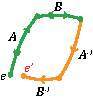
\includegraphics[width=0.4\columnwidth]{simple_Lie_figure.pdf}
  \caption{Geometric intuition of Lie theory. Initialized at point $e$,
  consider \emph{actions} $\mbf{A}$ and $\mbf{B}$ sequentially,
  and \emph{undo} actions $\mbf{B}^{-1}$ then $\mbf{A}^{-1}$.
  Composition of actions $\mbf{A}\mbf{B}\mbf{B}^{-1}\mbf{A}^{-1}$ would return to $e$.
  However,  \emph{switching} the order of undoing,
 by using $\mbf{A}\mbf{B}\mbf{A}^{-1}\mbf{B}^{-1}$, might not return to $e$,
incurring a discrepancy by landing on point $e'$.
  Lie theory provides a useful measure of the potential offset between $e$ and $e'$.}
  \label{fig:Informal_Lie}
\end{figure}
To answer this question, we leverage Lie theory 
\cite{iserles2000lie,agrachev2013control,robbin2022introduction}.
Geometrically, Lie theory measures the order-sensitivity of operations,
or the discrepancy caused by swapping the order of events (see \cref{fig:Informal_Lie} for an intuitive illustration).
This provides a hierarchy for classifying tasks and sequence models
under their \emph{degree} of order sensitivity as well as a method for quantifying approximation errors.

We show that order-symmetric models incur an unavoidable approximation error
when the task is order sensitive.
We then highlight increasing depth as a mechanism that
extends the expressivity of parallelizable sequence models, decreasing this approximation error.
Overall, our work characterizes depth-dependent error-expressivity behavior, and provides 
guidance for model choice based on the task structure.

\section{Mathematical Preliminaries}
\label{sec:math_prelim}
Here we introduce the mathematical framework used throughout the paper.
We highlight concepts formalizing order sensitivity and approximation error that will be used to establish our theories in \cref{sec:theory}.
Readers primarily interested in the main results and their practical implications may wish to proceed directly to \cref{sec:theory} and \cref{sec:exp}.

\subsection{Lie groups and Lie algebras}
\label{sec:LieAlgebra}
A \emph{Lie group} $G$ is a smooth manifold equipped with a group structure under smooth multiplication.
Its tangent space at the identity characterizes an associated \emph{Lie algebra} $\fr{g}$.
Generally, a Lie algebra is a vector space $\fr{g}$ equipped with a bilinear and antisymmetric Lie bracket operation $[\cdot, \cdot]: \fr{g} \times \fr{g} \to \fr{g}$ that satisfies the Jacobi identity:
\begin{equation*}
    [[X,Y],Z] = [X,[Y,Z]] - [Y,[X,Z]],
    \quad X,Y,Z \in \fr{g}.
\end{equation*}
A canonical example of the Lie bracket is a matrix commutator.
For matrices
$\mbf{A}, \mbf{B} \in \bb{R}^{n \times n}$,
the Lie bracket corresponds to the matrix commutator $[\mbf{A},\mbf{B}] = \mbf{A}\mbf{B} - \mbf{B}\mbf{A}$.

Given a vector space spanned by a collection of vector fields $\mcal{F}:= \{F_i\}$, the smallest Lie algebra is denoted as $\text{Lie}(\mcal{F})$ \cite{iserles2000lie}.
Unless otherwise mentioned, Lie algebras are finite-dimensional over $\bb{R}$.

\paragraph{Classes of Lie algebras}
Here we classify Lie algebras based on their \emph{degree} of order sensitivity.
The \emph{derived} series of $\fr{g}$ is the inductive sequence of commutator ideals:
\begin{equation*}
    \fr{g}^{(0)} = \fr{g},
    \quad
    \fr{g}^{(i)} = [\fr{g}^{(i-1)},\fr{g}^{(i-1)}].
\end{equation*}
If $\fr{g}^{(j)} = 0$ with the smallest finite number $j$, $\fr{g}$ is classified as a \emph{solvable} Lie algebra with derived length $j$.
Similarly, the \emph{lower central} series of $\fr{g}$ is a sequence of ideals spanned by nested commutators:
\begin{equation*}
    \fr{g}^0 = \fr{g},
    \quad
    \fr{g}^i = [\fr{g},\fr{g}^{i-1}].
\end{equation*}
If $\fr{g}^c = 0$ with the smallest finite number $c$, $\fr{g}$ is \emph{nilpotent} with class $c$.
An \emph{abelian} Lie algebra is the special case with $[\fr{g},\fr{g}]=0$ \cite{hall2013lie}.

These Lie algebras are related by a structural hierarchy.
Abelian Lie algebras are nilpotent, and all nilpotent Lie algebras are solvable.
A solvable Lie algebra can be constructed by a
\emph{tower} of abelian algebra extensions (\cref{app:rem_solvable_k_tower}).
Extension is formally introduced in \cref{app:subsubsec_extensionprelim}.
\subsection{State-space models and the Lie equation}
\label{sec:LPVsystem}
To connect Lie theory with sequence models, we formalize state-space models
as controlled dynamical systems on Euclidean space (\cref{app:control_detail}).
We will observe how the Lie algebra characterizes a dynamical system.
\begin{definition}[State space model]
\label{def:staticLPVsystem}
A \emph{state space model} (SSM) is an affine vector field
on Euclidean \emph{state space} $\mcal{M} = \bb{R}^n$
and \emph{input space} $\mcal{X}$
such that:
\begin{equation}
\label{eq:vectorstateODE}
F_x: \mcal{M} \to T\mcal{M},
\quad F_x(h) := \mbf{A}(x) h + \mbf{b}(x).
\end{equation}
$\mbf{A}: \mcal{X} \to \bb{R}^{n \times n}$ and $\mbf{b}: \mcal{X} \to \bb{R}^n$ are real analytic \cite{sontag2013mathematical}.
We call $\mbf{A}$ the \emph{generator} of the SSM.
We denote the SSM as $\mbf{S}$, and $\dim \mbf{S} := \dim \mcal{M}$.
\end{definition}
We assume SSMs satisfy mild regularity conditions (\cref{app:control_detail}).
With a locally bounded and integrable input path $x(\cdot): [0,T] \to \mcal{X}$,
one can reintroduce time in \cref{eq:vectorstateODE} and construct an ODE form.
We say that an SSM is \emph{initialized} when the initial state $h(0)$ is fixed.

In what follows, we focus on the dynamics generated by $\mbf{S}$.\footnote{
Our theory focuses on the state evolution. When outputs matter, we equip $\mbf{S}$ with
the \emph{output space} $\mcal{Y}$ and real analytic output map $g$ \cite{sontag2013mathematical}.}
\begin{definition}[State-transition matrix]
\label{def:Phi}
    The state-transition matrix $\Phi$
    is an evolution operator of the homogeneous flow:
    \begin{equation}
        \label{eq:STM}
        \Phi_x(t,0) = \mcal{T} \exp \int_0^t \mathbf{A}(x(\tau)) \; d\tau,
    \end{equation}
    where $\mcal{T} \exp$ denotes the chronological (time-ordered) exponential \cite{agrachev2013control, sontag2013mathematical}.
\end{definition}
\paragraph{From state-centric to flow-centric view}
\label{sec:flow_centric_realization}
Rather than tracking a single state, one can consider tracking entire \emph{flows}.
This perspective bridges Lie algebras and SSMs.

Let us note some key features of $\Phi(t,0)$:
\begin{equation}
\label{eq:PhiFeature}
    \dot{\Phi}(t,0) = \mbf{A}(x(t))\Phi(t,0),
    \quad
    \Phi(0,0) = I.
\end{equation}
It turns out that this is a \emph{Lie equation} \cite{iserles2008magnus}:
\begin{definition}[Controlled Lie equation]
\label{def:LieGroupEquation}
A linear controlled Lie equation is a matrix ODE:
\begin{equation}
\label{eq:LieGroupEquation}
    \dot{\Psi}(t) := \mbf{A}(x(t)) \Psi(t),
    \quad
    \Psi(0) = I.
\end{equation}
where $\text{Lie}(\{\mbf{A}(x)\}) = \fr{g} \subseteq \fr{gl}(n,\bb{R})$, $\Psi \in G \subseteq \G{GL}{n,\bb{R}}$ and the Lie group $G$ locally integrates $\fr{g}$.
\end{definition}
It is immediately clear that \cref{eq:PhiFeature} aligns with \cref{def:LieGroupEquation}:
$\Phi$ can be considered as a local curve on $G$.
Therefore, the controlled linear Lie equation is a \emph{flow-centric} ODE,
tracking all sets of local evolutions rather than a single state \cite{jurdjevic1972control}.

As $\fr{g}$ locally characterizes $\Phi$,
we classify SSMs with the algebraic class of $\fr{g}$
and, for short, denote it $\mbf{S}_\fr{g}$.
We map SSMs to its Lie equations via \emph{lifting}.
\begin{definition}[Lift]
    Consider an $\mbf{S}_\fr{g}$ with initial state $h_0$.
    Its lifted Lie equation extends \cref{eq:LieGroupEquation}
    with augmented flow space $G \times \mcal{M}$.
    For $\Psi \in G, \: h_0 \in \mcal{M}$:
    \begin{equation*}
        \dot{\Psi}(t) = \mbf{A}(x(t))\Psi(t),
        \
        \dot{h}(t) = 0,
        \
        \bigl( \Psi(0), h(0) \bigr) = \bigl( I, h_0 \bigr).
    \end{equation*}
\end{definition}
\paragraph{Restricted SSM}
\label{sec:main_affine_vector_field}
As an umbrella term, we say $\mbf{S}_\fr{g}$ is \emph{restricted}
if $\text{Lie}(\{\mbf{A}(x)\})$ is abelian.
Although inhomogeneous SSMs can be order-sensitive due to the translation term, $\mbf{b}$,
we observe that SSM expressivity is mostly determined by the generator, $\mbf{A}$.\footnote{
One can absorb $\mbf{b}$ via \emph{homogenization} and treat an affine SSM
as a homogeneous SSM \cite{krener1977decomposition}. Details in \cref{app:bridge_to_general_LPV}.}
If not restricted, $\mbf{S}_\fr{g}$ is \emph{general}.
\subsection{Simulation and error}
\label{par:sim_min_main}
Studying expressivity of a model class is tied to \emph{simulation}:
whether one system can reproduce another's behavior \cite{liu2022transformers}.
Analogously, we use a \emph{state-based} notion of simulation.\footnote{
In this context, we assume the target system $\mbf{S}_1$ is \emph{minimal}.
Minimality is formally treated in \cref{app:min_detail}.}

Informally, we say $\mbf{S}_0$ simulates $\mbf{S}_1$
if a smooth surjective submersion $\varphi: \mcal{M}_0 \to \mcal{M}_1$ maps
$\mbf{S}_0$ state evolution to $\mbf{S}_1$ states under any admissible inputs.
When exact simulation is impossible, we quantify the approximation error.\footnote{
Formally introduced in \cref{app:sim_detail} with \emph{simulation error}.}
Note that lifted the Lie equation simulates the original initialized SSM,
\begin{equation}
\label{eq:flow_to_state_submersion}
    \varphi: G \times \mcal{M} \to \mcal{M},
    \quad
    \varphi\bigl( \Phi, h \bigr) = \Phi h,
\end{equation}
so that $h(t) = \varphi\bigl( \Phi(t,0), h(0) \bigr) = \Phi(t,0)h(0)$.
\paragraph{Magnus expansion}
\label{par:MagnusExpansion}
Given the Lie-algebraic perspective of SSMs,
we now introduce a quantitative tool for the simulation error.
The \emph{Magnus expansion} decomposes $\Phi$ via exponential of
iterated Lie brackets (\cref{app:CDE}),
providing an explicit measure of order-relevant errors.
\begin{definition}[Commutator mass]
\label{def:commutator_mass}
    Given a fixed input path $x$ over the interval $[0,T]$,
    we define \emph{commutator mass} of $\mbf{S}$
    as the norm of the second-order Magnus term, $\|\Omega_2\|$:
    \begin{align}
    \label{eq:omega_2}
        \Omega_2
        &= \frac{1}{2}
        \int_0^T dt_1
        \int_0^{t_1} dt_2
        [\mbf{A}(x(t_1)), \mbf{A}(x(t_2))]
        \\
        &= \frac{1}{4}\iint_{[0,T]^2}
        \text{sgn}(t_1 - t_2)
        [\mathbf{A}(x(t_1)), \mathbf{A}(x(t_2))]
        \, dt_1 dt_2. \nonumber
    \end{align}
\end{definition}
We work on small windows in which the Magnus series converges.
Long horizon behavior for large $T$ is constructed by the composition of small time partitions \cite{sontag2013mathematical}:
\begin{equation}
\label{eq:flow_composition}
    \Phi(T,0) = \prod_{i=0}^n \Phi(t_{i+1}, t_i),
    \quad
    t_0=0,
    \
    t_{n+1}=T.
\end{equation}
\subsection{Deep structure}
Most practical applications of artificial neural networks leverage deep layered structures with additional pointwise computation (e.g. MLP) between layers. To extend our theory, here we discuss dynamical systems with deep layered structure  \cite{krener1977decomposition}.
\begin{definition}[Deep SSM]
\label{def:stacking}
    The \emph{cascade} of $\mbf{S}_0$ and $\mbf{S}_1$ is
    defined with a smooth map $v: \mcal{M}_0 \times \mcal{X} \to \mcal{X}_1$:
    \begin{align*}
        \mcal{M} &\cong \mcal{M}_0 \times \mcal{M}_1, \: x_1(t) = v(h_0(t), x(t)) \\
        \dot{h}_0(t) &= \mbf{A}_0(x(t))h_0(t) + \mbf{b}_0(x(t)) \\
        \dot{h}_1(t) &= \mbf{A}_1(x_1(t))h_1(t) + \mbf{b}_1(x_1(t)).
    \end{align*}
     A deep SSM is obtained inductively:
     \begin{align*}
        x_i(t) &= v_i(h_{i-1}(t), \cdots, h_0(t), x(t)),
        \quad
        x_0(t) = x(t) \\
        \dot{h}_i(t) &:= \mbf{A}_i(x_i(t)) h_i(t) + \mbf{b}_i(x_i(t)).
     \end{align*}
     where $v_i: \Bigl( \prod_{j=0}^{i-1} \mcal{M}_j \Bigr) \times \mcal{X} \to \mcal{X}_i$ is smooth.

     We refer to each local SSM as the $i$-th layer.
     An $L$-layer SSM is said to be restricted when all of its layers are restricted.
     This convention applies to the other classes as well.
\end{definition}
\subsection{Word problems}
\label{sec:intro_word_problems}
Here we briefly introduce \emph{word problems}, one of the standard test beds for sequence model expressivity.
We also use it in the experimental \cref{sec:exp}.
For a formal introduction, we refer to \cref{app:def_formal_wordproblem}.

Informally, a word problem is defined for a finitely generated group
\footnote{More generally, word problems can be defined for a monoid or group given a finitely generating alphabet set.}
\cite{liu2022transformers, merrill2024illusion}.
We treat elements of the generating set as \emph{alphabet symbols},
and the product of a sequence of these symbols as a \emph{word}.
Under the group composition rule, each word evaluates to a group element.
The word problem asks whether one can evaluate arbitrary words to the corresponding group elements.

From a computational perspective, the word problem can be viewed as a symbolic state-tracking task.
As symbols arrive sequentially, the model must update an internal state according to the group multiplication rule
and determine the resulting group element.

Let us provide a tangible example.
Consider each \emph{alphabet symbol} as a \emph{primitive action}, such as permutation, rotation, or a state transition operation (\cref{fig:Informal_Lie}).
A \emph{word} is then a sequence of \emph{action commands} evaluated by composing primitive actions in the given order.
A sequence of matrix multiplication, or a rollout in a Markov decision process (MDP) with action-conditioned state transition, provide examples of word evaluation.

The algebraic complexity of word problems is therefore rich and well-defined.
When the chosen finite group is abelian, the corresponding word problem is inherently order-symmetric.
In contrast, swapping alphabet orders in non-abelian groups can change evaluation,
introducing order-sensitivity.
We provide the class of exemplary word problems and related concrete problems in \cref{tab:words}.
\begin{table}[t]
\setlength{\tabcolsep}{0.3em}
  \caption{Class of representative word problems.}
  \vspace{-3mm}
  \label{tab:words}
  \begin{center}
    \begin{small}
        \begin{tabular}{lcccr}
          \toprule
          Class  & Group example         & Related problems\\
          \midrule
          Abelian    & $C_2, C_3, C_{60}, SO(2)$ & Parity; Cyclic gridworld \\ 
         Nilpotent & $D_8, H_3$ & Quantum spin \\
          Solvable    & $S_3, A_4, S_4$ & 2D affine transformation \\
          Non-solvable    & $A_5, S_5, SO(n\ge3)$ & Rubik's cube; 3D rotation\\
          \bottomrule
        \end{tabular}
    \end{small}
  \end{center}
  \vskip -0.1in
\end{table}

\section{Theory}
\label{sec:theory}
Our theory has two major parts.
For single-layer models, \cref{thm:sim_error} derives a simulation error bound.
Then, \cref{thm:Kstacks} provides theoretical ground on how depth extends expressivity.
\cref{col:nilpotentization} and \cref{col:logdepth}
explain how depth mitigates simulation error
and construct an upper bound for depth-dependent expressivity errors.
\subsection{Expressivity bounds of a single layer}
\label{sec:theory_single_layer}
In the single-layer case, we align our formulation with prior work \cite{merrill2024illusion, liu2022transformers, anonymous2025the} and constructively provide an error bound.
For clarity, here we use $\mbf{S}$ for general SSMs,
and $\hbf{S}$ for restricted SSMs.
\begin{lemma}
\label{lem:sim_impossible}
No abelian $\hbf{S}$ can simulate a general SSM.
\end{lemma}
Proof is provided in \cref{app:sim_impossible_proof}.
\begin{theorem}
\label{thm:sim_error}
    Consider a restricted $\hbf{S}$ that approximates $\mbf{S}$.
    Under mild assumptions, there exists an input path $x$ on small time interval
    that incurs simulation error scaling with the commutator mass $\|\Omega_2\|$ of $\mbf{S}$.
    The error can
    accumulate over long horizon and scale with sequence length.
\end{theorem}
Proof is provided in \cref{app:sim_error_proof}.

\begin{proof}[Proof sketch]
The order symmetry generates irreducible
order-sensitive error, which locally scales with the commutator mass.
Intuitively, consider applying the action set in \cref{fig:Informal_Lie} iteratively.
The local discrepancy between $e$ and $e'$ could accumulate.
\end{proof}
\subsection{Expressivity bounds at deep structure}
\label{sec:theory_multi_layer}
Here we consider deep restricted SSMs
and discuss how depth mitigates their expressivity limits.
\begin{proposition}
\label{lem:stackderivedlength}
    Restricted $k$-layer SSMs are solvable with at most $2k$ derived length.
    % Abelian $k$-layer SSMs are limited at most $k$.
    Abelian $k$-layer SSMs are
    solvable with at most $k$ derived length.
\end{proposition}
Proof is provided in \cref{app:stackderivedlength_proof}.

\cref{lem:stackderivedlength} points out that any finite-depth restricted SSM is limited to be solvable.
Indeed, \citet{merrill2024illusion} and \citet{muca2024theoretical}
reported that scalable sequence models need
\emph{infinite} depths to be fully expressive.
\begin{theorem}
\label{thm:Kstacks}
    Consider $\mbf{S}_\fr{g}$ such that the derived length of $\fr{g}$ is $k$.
    Then, there exists an abelian $k$-layer SSM plus smooth output map
   that simulates $\mbf{S}_\fr{g}$.
\end{theorem}
Proof is provided in \cref{app:sub_proofKstacks}.

\cref{thm:Kstacks} shows that deep abelian SSMs are quite powerful as the deep structure permits abelian SSMs to generate order-sensitive solvable flows.\footnote{
Our proof technique analogously applies to general finite-dimensional Lie algebra extension,
check \cref{rem:non_abelian_extension_generalization}.}
Altogether, \cref{thm:Kstacks} provides
intuition for how the depth of a system characterizes its algebraic class.
\begin{remark}[Practical implication of \cref{thm:Kstacks}]
We again use MDP to construct a tangible intuition. As noted in \cref{tab:words}, different orders of action execution generally lead to different action-dependent transition matrices.
    Except in simple cases (e.g. cyclic gridworld), modeling order-sensitive dynamics is critical to whether a sequence model can represent an MDP or serve as a learned \emph{world model} in model-based reinforcement learning \cite{chen2022transdreamer}.
    
    Intuitively, \cref{thm:Kstacks} provides a concrete answer to how many layers are required to represent a \emph{composition} of actions with the correct transition structure.
    In theory, each layer tracks a collection of \emph{commuting} components of dynamics, whose composition reconstructs non-commuting transitions.
    This mirrors the construction of Lie algebra extensions and tower of abelian extensions.
    
    Under piecewise-constant inputs (or any suitable discretization), the SSMs in our theory can be considered as discrete-time sequence models.
    In practice, parallelizable sequence models impose additional structural biases to achieve high stability or  scalability.
    Therefore, we empirically test how models behave in \cref{sec:exp}.
\end{remark}
\vspace{2mm}
\cref{thm:Kstacks} naturally maps to the well-known control theory literature.
For concrete measure, we introduce the \emph{generator mass}.
Given an input path over the short interval $[0,T]$,
we define the local \emph{generator mass} of $\mbf{S}$:
    \begin{equation*}
        \epsilon = \int_0^T \|\mbf{A}(x(t))\| \, dt < 1,
    \end{equation*}
assuming $\epsilon < 1$ without loss of generality for short enough $[0,T]$.
leading to the following approximation result.
\begin{corollary}
\label{col:nilpotentization}
    For non-solvable $\mbf{S}_\fr{g}$, there exists an abelian $k$-layer SSM whose
    local simulation error scales with $\mcal{O}(\epsilon^{2^{k-1}+1})$.
\end{corollary}
Proof is provided in \cref{app:sub_proof_nilpotentization}.
Note that \cref{thm:sim_error} corresponds to $k=1$. The commutator mass, $\|\Omega_2\|$, scales in $\mcal{O}(\epsilon^2)$.

\cref{col:nilpotentization} is a promising result: although algebraically obstructed,
deep structure exponentially mitigates the order-sensitive error.
The local error can again extends to long horizon via \cref{eq:flow_composition}.

The piecewise-constant approximation lemma bridges us back to
practical discrete-time realization \cite{krener1977decomposition}.
\begin{proposition}
\label{col:logdepth}
    Any word problem with word length bounded by $T$
    can be simulated by an
    abelian deep SSM with at most $\bigl(\lceil \log_2T \rceil + 1\bigr)$-layers and a smooth output map.\footnote{
Similar logarithmic depth result for transformers and semiautomata was reported in Theorem 1 of \citet{liu2022transformers},
and empirically observed in \citet{hu2024limitation}.
}
\end{proposition}
Proof and a formal introduction of the word problem are provided in \cref{app:sub_proof_logdepth}.

\cref{col:logdepth} provides an explicit upper bound on the depth required to simulate discrete, finite-length sequences.
Many practical applications, such as \emph{model predictive control},
rely on constant-length sequence generation \cite{hafner2019learning}.
Therefore, despite of their brittleness to generalization \cite{liu2022transformers},
finite-depth scalable sequence models may suffice in practice.
Note that \cref{col:logdepth} provides the worst-case depth upper bound, imposing minimal equivalence relation on words. In practice, much shallower SSMs may successfully simulate a given word problem when the finite group is well-structured.
For example, a single layer abelian SSM suffices to simulate an abelian word problem for any $T$.

Lastly, we note that solving the bounded length word problem can come at a cost of significant state expansion.
\begin{corollary}
\label{col:logdepth_state}
Consider an alphabet of size
$|\mcal{A}| = n$ and word length bounded by $T$.
Then, the total state space dimension of the abelian deep SSM constructed in \cref{col:logdepth} exponentially grows in $T$ for fixed $n$ with asymptotic order $\mcal{O}(n^T/T)$.
\end{corollary}
Proof is provided in \cref{app:sub_proof_logdepth_state}. Again, this is a worst-case width upper bound following the construction of \cref{col:logdepth}.
Depending on the structure of the word problem, the required width can be much smaller.
For example, \cref{thm:Kstacks} yields an abelian deep SSM which can exactly simulate some word problems with fixed state size, not growing in $T$.

Taken together, \cref{col:logdepth} and \cref{col:logdepth_state} clarify how depth and width (i.e. state space dimension) plays a role in constant length simulation. Logarithmic depth growth suffices to lift the algebraic obstruction at sequence length $T$, while exact simulation still requires a substantial state space expansion.
Importantly, depth and width are orthogonal here.
The construction in \cref{col:logdepth}
can also be realized with a single-layer nilpotent SSM.
However, its required state space dimension is still characterized as in \cref{col:logdepth_state}.

\begin{remark}[Conjecture on restricted SSMs]
\label{rem:conjecture_restricted_limits}
    As shown in \cref{thm:sim_error}, restricted SSMs do not substantially extend expressivity beyond abelian SSMs. Although restricted SSMs can be order-sensitive (\cref{sec:main_affine_vector_field}), their strong structural constraints prevent them from simulating general SSMs with a single layer.
    Motivated by this observation, we conjecture that the advantage of restricted layers over abelian layers is limited. In particular, we conjecture the existence of solvable $\mbf{S}_\fr{g}$ whose derived length is $k+1$, but cannot be simulated by any restricted $k$-layer SSM.
\end{remark}

\section{Experiments}
\label{sec:exp}
Here we experimentally illustrate our theoretical results by evaluating representative parallelizable sequence models on various state-tracking problems.  We examine symbolic word problems (\cref{sec:exp_wp}) covering those that are abelian ($C_2$, $C_3$), nilpotent ($D_8$, $H_8$), solvable ($S_3$, $S_4$) or non-solvable ($A_5$), as well as a physical rotation prediction problem based on $A_5$ (\cref{sec:exp_rotation}).

Regarding the model architecture, in addition to the basic transformer \citep{trafo}, we study three types of diagonal structured SSMs: GLA \citep{YangWSPK24}, signed Mamba \citep{grazzi2024unlocking}, and AUSSM \citep{karuvally2025bridging}.
Generators of each models are structured as positive, signed, and complex diagonal matrices, respectively.
These architectures can be thought of discretized versions of restricted SSMs in our theory.
Additionally, we also report on the performance of DeltaProduct \citep{siems2025deltaproduct} as a general SSM class
that can solve the chosen tasks in theory and practice.

\begin{table}[t]
\setlength{\tabcolsep}{0.4em}
\caption{Length generalization performance measured as sequence-level accuracy for various categories of word problems. Models are trained on length 128 and tested on 256. $L$ denotes the number of layers. DeltaProduct uses the theoretically necessary number of Householder products depending on the problem. The blue color cell highlights perfect generalization.
Hyper-parameter search space can be found in Appendix \ref{app:exp_wp}.
The number of training sequences is 500K for all tasks, except for $C_2$ which uses 100K.
}
\vspace{-2mm}

\label{tab:word_problem}
\begin{center}
\small
\begin{tabular}{lccccccc}
\toprule
& & \multicolumn{2}{c}{Abelian} & \multicolumn{2}{c}{Nilpotent} & \multicolumn{2}{c}{Solvable}  \\
 \cmidrule(r){3-4} \cmidrule(r){5-6} \cmidrule(r){7-8} 
Model   & $L$      & \multicolumn{1}{c}{$C_2$} & \multicolumn{1}{c}{$C_3$} & \multicolumn{1}{c}{$D_8$} & \multicolumn{1}{c}{$H_3$} & \multicolumn{1}{c}{$S_3$} & \multicolumn{1}{c}{$S_4$} \\ \midrule
Transformer  & 1 & 0.00 & 0.00 & 0.00 & 0.00 & 0.00 & 0.00 \\ \midrule
(+-only) Mamba & 1 & 0.00 & 0.00 &  0.00  & 0.00 & 0.00 & 0.00  \\  \midrule
(+-only) GLA & 1 &  0.00  & 0.00 & 0.00 & 0.00 & 0.00 & 0.00 \\ 
                  & 2 &  0.00  & 0.00 & 0.00 & 0.00 & 0.00 & 0.00  \\ \midrule 
Signed Mamba          & 1 & \cellcolor{blue!10} 1.00 & 0.00 & 0.00 &  0.00  & 0.00 & 0.00   \\  
& 2 & \cellcolor{blue!10} 1.00 & 0.00 & \cellcolor{blue!10} 1.00 & \cellcolor{blue!10} 1.00 & \emph{0.19} & 0.00 \\  \midrule
AUSSM    & 1 & \cellcolor{blue!10} 1.00 & \cellcolor{blue!10} 1.00 & 0.00 &  0.00  & 0.00 & 0.00    \\  
    & 2 & \cellcolor{blue!10} 1.00 & \cellcolor{blue!10} 1.00 & 0.00 & 0.00 & 0.00 & 0.00 \\  \midrule
DeltaProduct & 1 & \cellcolor{blue!10} 1.00 &  \cellcolor{blue!10}  1.00 & \cellcolor{blue!10} 1.00  & \cellcolor{blue!10} 1.00 & \cellcolor{blue!10} 1.00 &\cellcolor{blue!10} 1.00   \\
\bottomrule
\end{tabular}
\end{center}
\vspace{-6mm}
\end{table}

\subsection{Length Generalization on Solvable Word Problems}
\label{sec:exp_wp}
Here we evaluate performance on symbolic state-tracking problems, formalized as word problems (WPs) with chosen finite groups.
We selected word problems for each class and trained sequence models to confirm each models' algebraic capacity using various depths.\looseness=-1

Following prior work \citep{merrill2024illusion,siems2025deltaproduct}, we formulate a word problem as a sequence labeling task.
Each sequence consists of tokens with each token representing a group element.
At each position in a sequence to be read from left to right, we have a target label/token corresponding to the group element obtained by composing symbols in the sequence so far.
The model is trained to predict the corresponding target label at each position.
Further experimental details can be found in Appendix \ref{app:exp_wp}.

We first evaluate the length generalization performance by training models on sequences of length 128 and testing them on length up to 256.
Results are shown in Table \ref{tab:word_problem}; and we break down the results as follows.

\textbf{Abelian WPs.}
We first evaluate models on abelian WPs as a smoke test.
Empirically, echoing prior work, we observe that transformer failed to model the simplest abelian word problems, $C_2$.
Similarly, positive diagonal only (denoted as +-only) GLA and Mamba did not perform well in $C_2$.
In contrast, Signed Mamba can solve $C_2$, while failing on $C_3$; and AUSSM succeeded at both $C_2$ and $C_3$.

\textbf{Nilpotent and Solvable WPs.}
We further evaluate models on more challenging WPs.
Theoretically, $D_8$, $H_3$, and $S_3$ requires at least two, while $S_4$ requires three, layers of \emph{abelian} SSMs.
Note that sequence models correspond to \emph{restricted} SSMs, and may solve $S_4$ in two layers. However, we conjectured that this would not be the case \cref{rem:conjecture_restricted_limits}.

Consistent with the prediction, none of the models except DeltaProduct successfully performed the task with a single layer.
With two layers, we observe that the inductive bias significantly influences model behavior.
Signed Mamba successfully learned $D_8$, a nilpotent task,
but only achieves partial generalization on the solvable task $S_3$.
In contrast, AUSSM fails to learn a generalizable solution for
non-abelian word problems under our experimental setting.

It remains an open question what hinders the performance of deeper models.
Still, several factors may offer some insights.
Our theory constructs on real arithmetic whereas empirical computation is on finite precision; the impact of finite precision is beyond the scope of the current work. 
Moreover, without further constraints, how gradient-based optimization shapes the solution is also unclear.
This points to the \emph{learnability} issue:
the practical learnability is influenced by the low-level inductive biases of
each model (i.e., the specific choice of state update rules), which are tangential to the expressivity theory.
For example, we empirically observe that, although Signed Mamba has a more restricted eigenvalue range than AUSSM,
empirically it performed better in the $2$-layer regime (see further comments on the trainability of AUSSM in Appendix \ref{app:exp_rotation}).

\begin{figure}[t]
    \begin{center}
        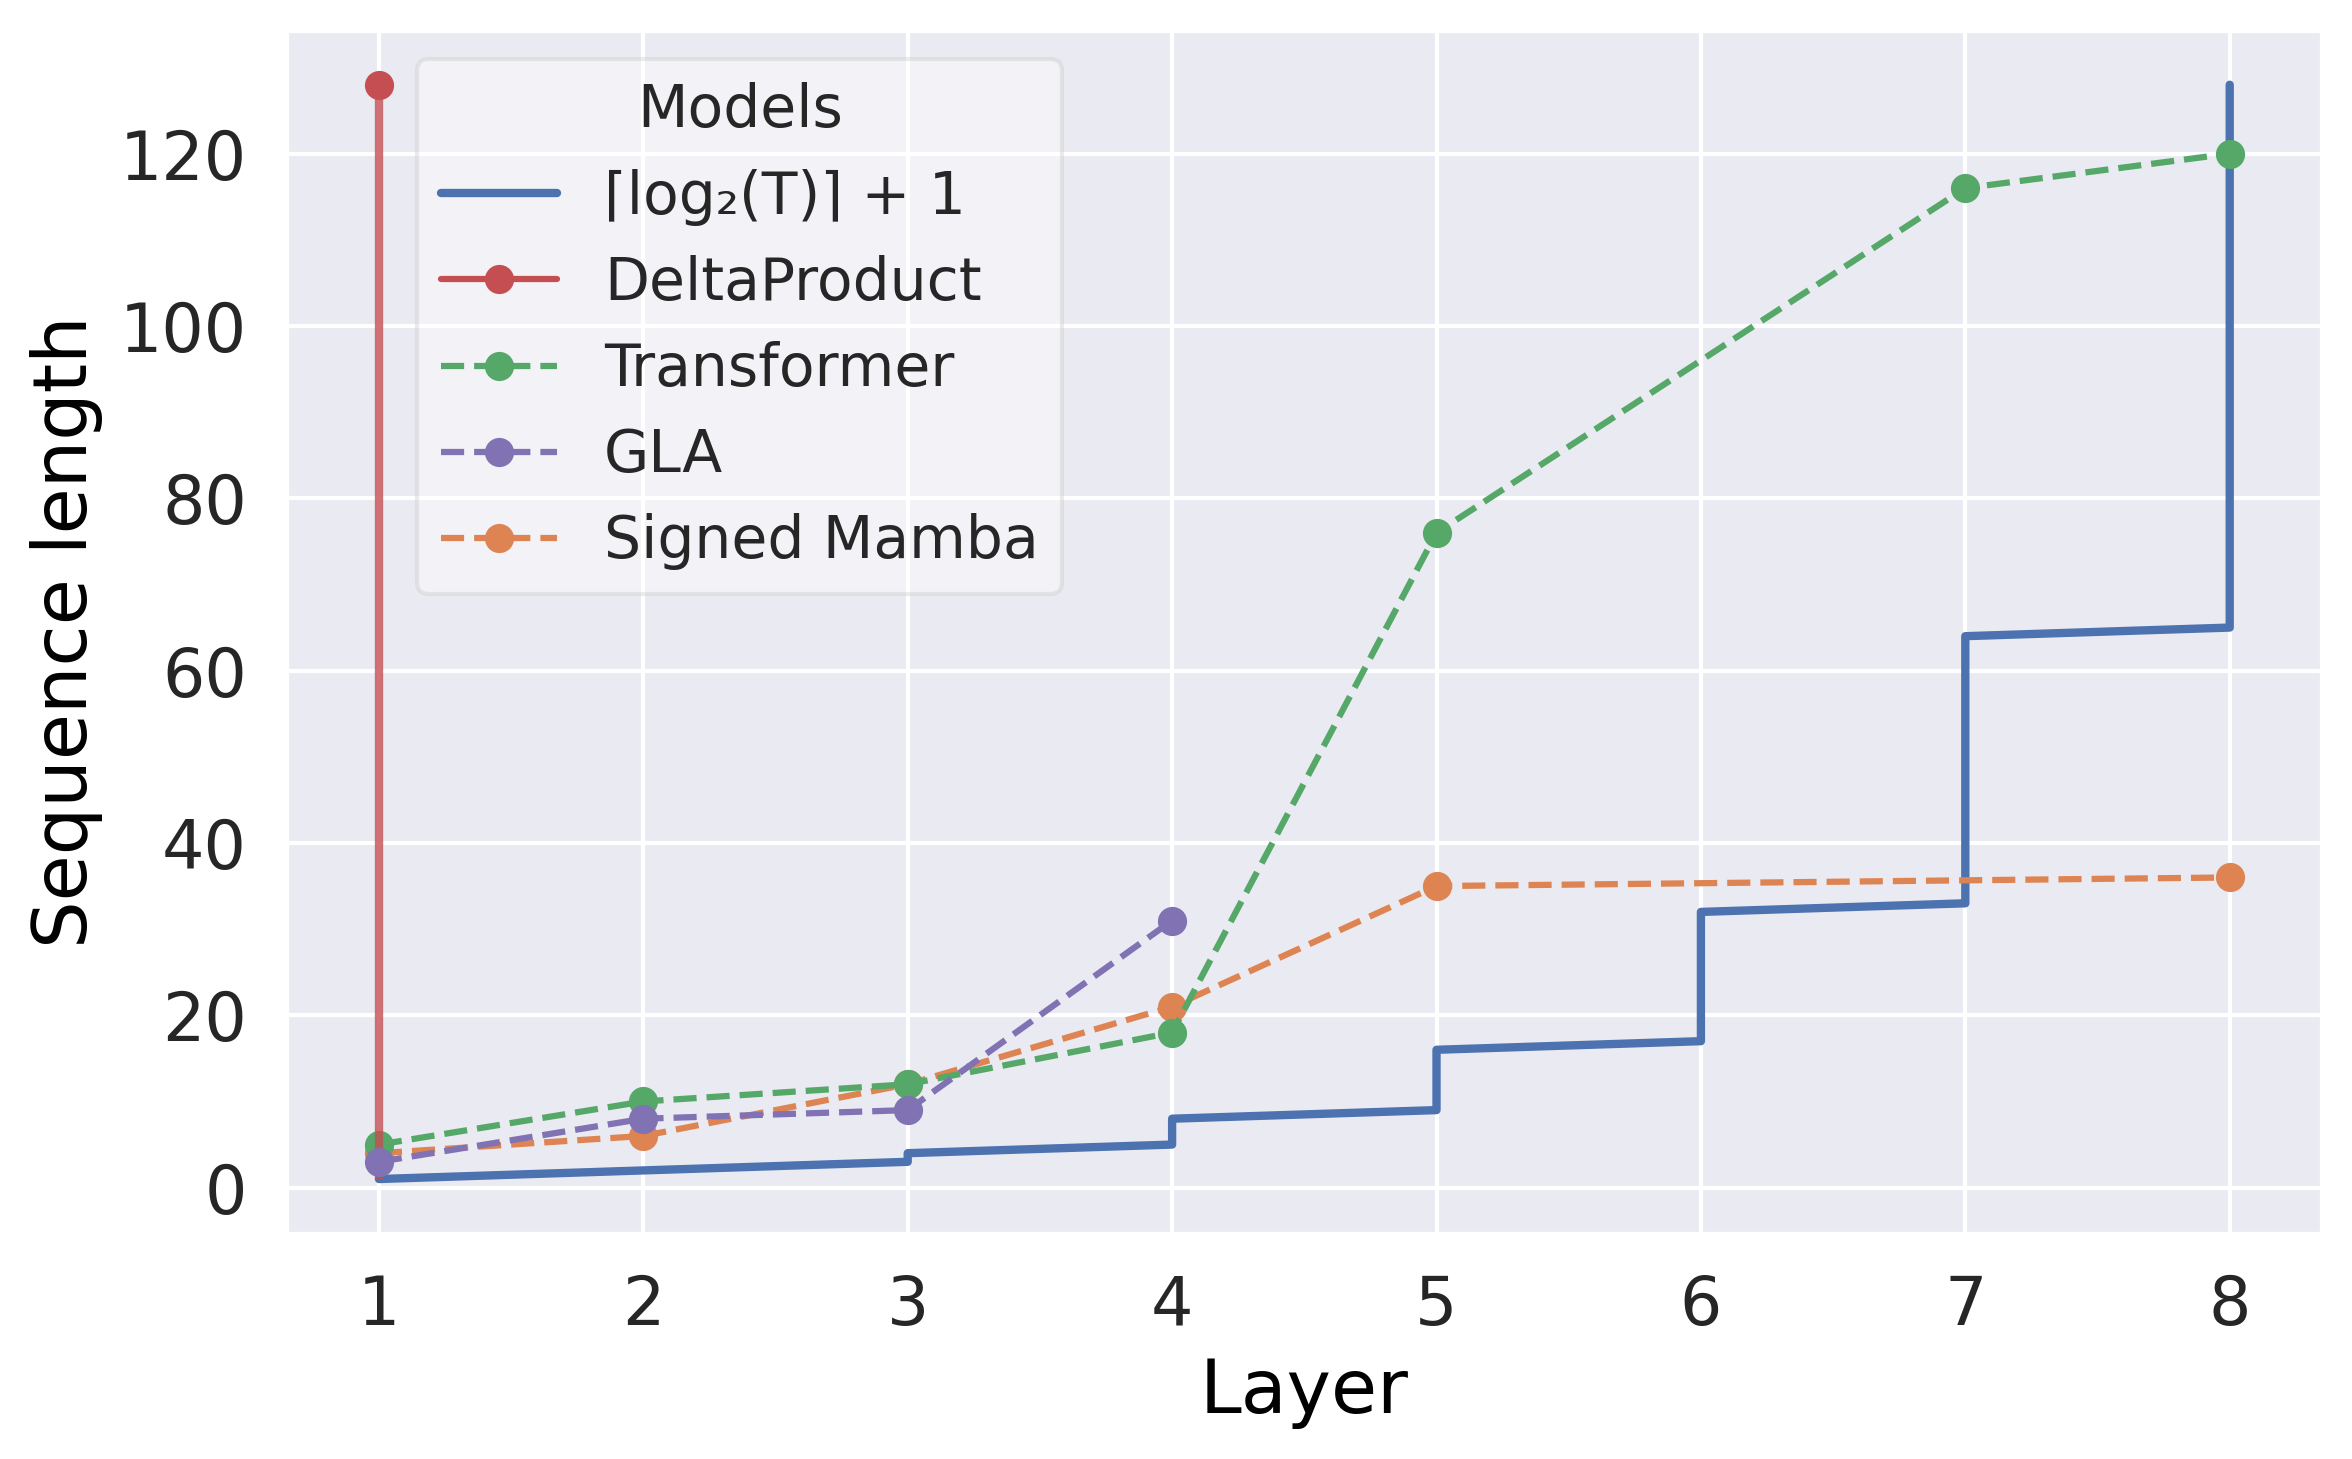
\includegraphics[width=1.0\columnwidth]{figures/seqlen_vs_depth_vertical.png}
        \caption{Maximum sequence length for each model with varying number of layers to achieve $>90\%$ sequence-level prediction accuracy on the training set of the word problem $A_5$. All models are trained on length up to 128. Deep models ($>$ 4 layers) that failed to achieve a longer sequence length than shallower models are not shown; deep GLA and signed Mamba models often fail to learn this task.  $T$ in the legend $\bigl(\lceil \log_2T \rceil + 1\bigr)$ is sequence length (i.e., y-axis).
}
        \label{fig:seqlen_vs_layer}
    \end{center}
\end{figure}


\subsection{Depth vs.~Length in Non-solvable Word Problems.}
Here we focus on $A_5$ as the simplest non-solvable word problem to illustrate how increasing the model depth enhances performance
beyond its expressivity range, in line with \cref{col:logdepth}.

Figure \ref{fig:seqlen_vs_layer} shows the maximum length of the sequence that the model can accurately predict for a given number of layers.
We chose the accuracy cutoff at $> 90\%$, and compared results to the theoretical depth upper bound provided at \cref{col:logdepth}.

We observe that transformer clearly benefits from depth.
By varying the number of layers from 1 to 8, transformer performance improves
following the trend of the theoretical bound (\cref{sec:theory}).
In the case of GLA and Signed Mamba, we observe a similar trend showing the benefit of depth, increasing from 1 up to depth 4 or 5.

However, we observe that deeper models are hard to train on this task; some of the deep models performed worse than shallower ones. 
This is again illustrative of the practical learnability issue discussed in the previous section.
In particular, the 8-layer Signed Mamba only slightly improves upon the 5-layer one (achieving length 36 vs.~35), which is less efficient than the bound expected by our theory.

\begin{figure*}[t]
    \begin{center}
        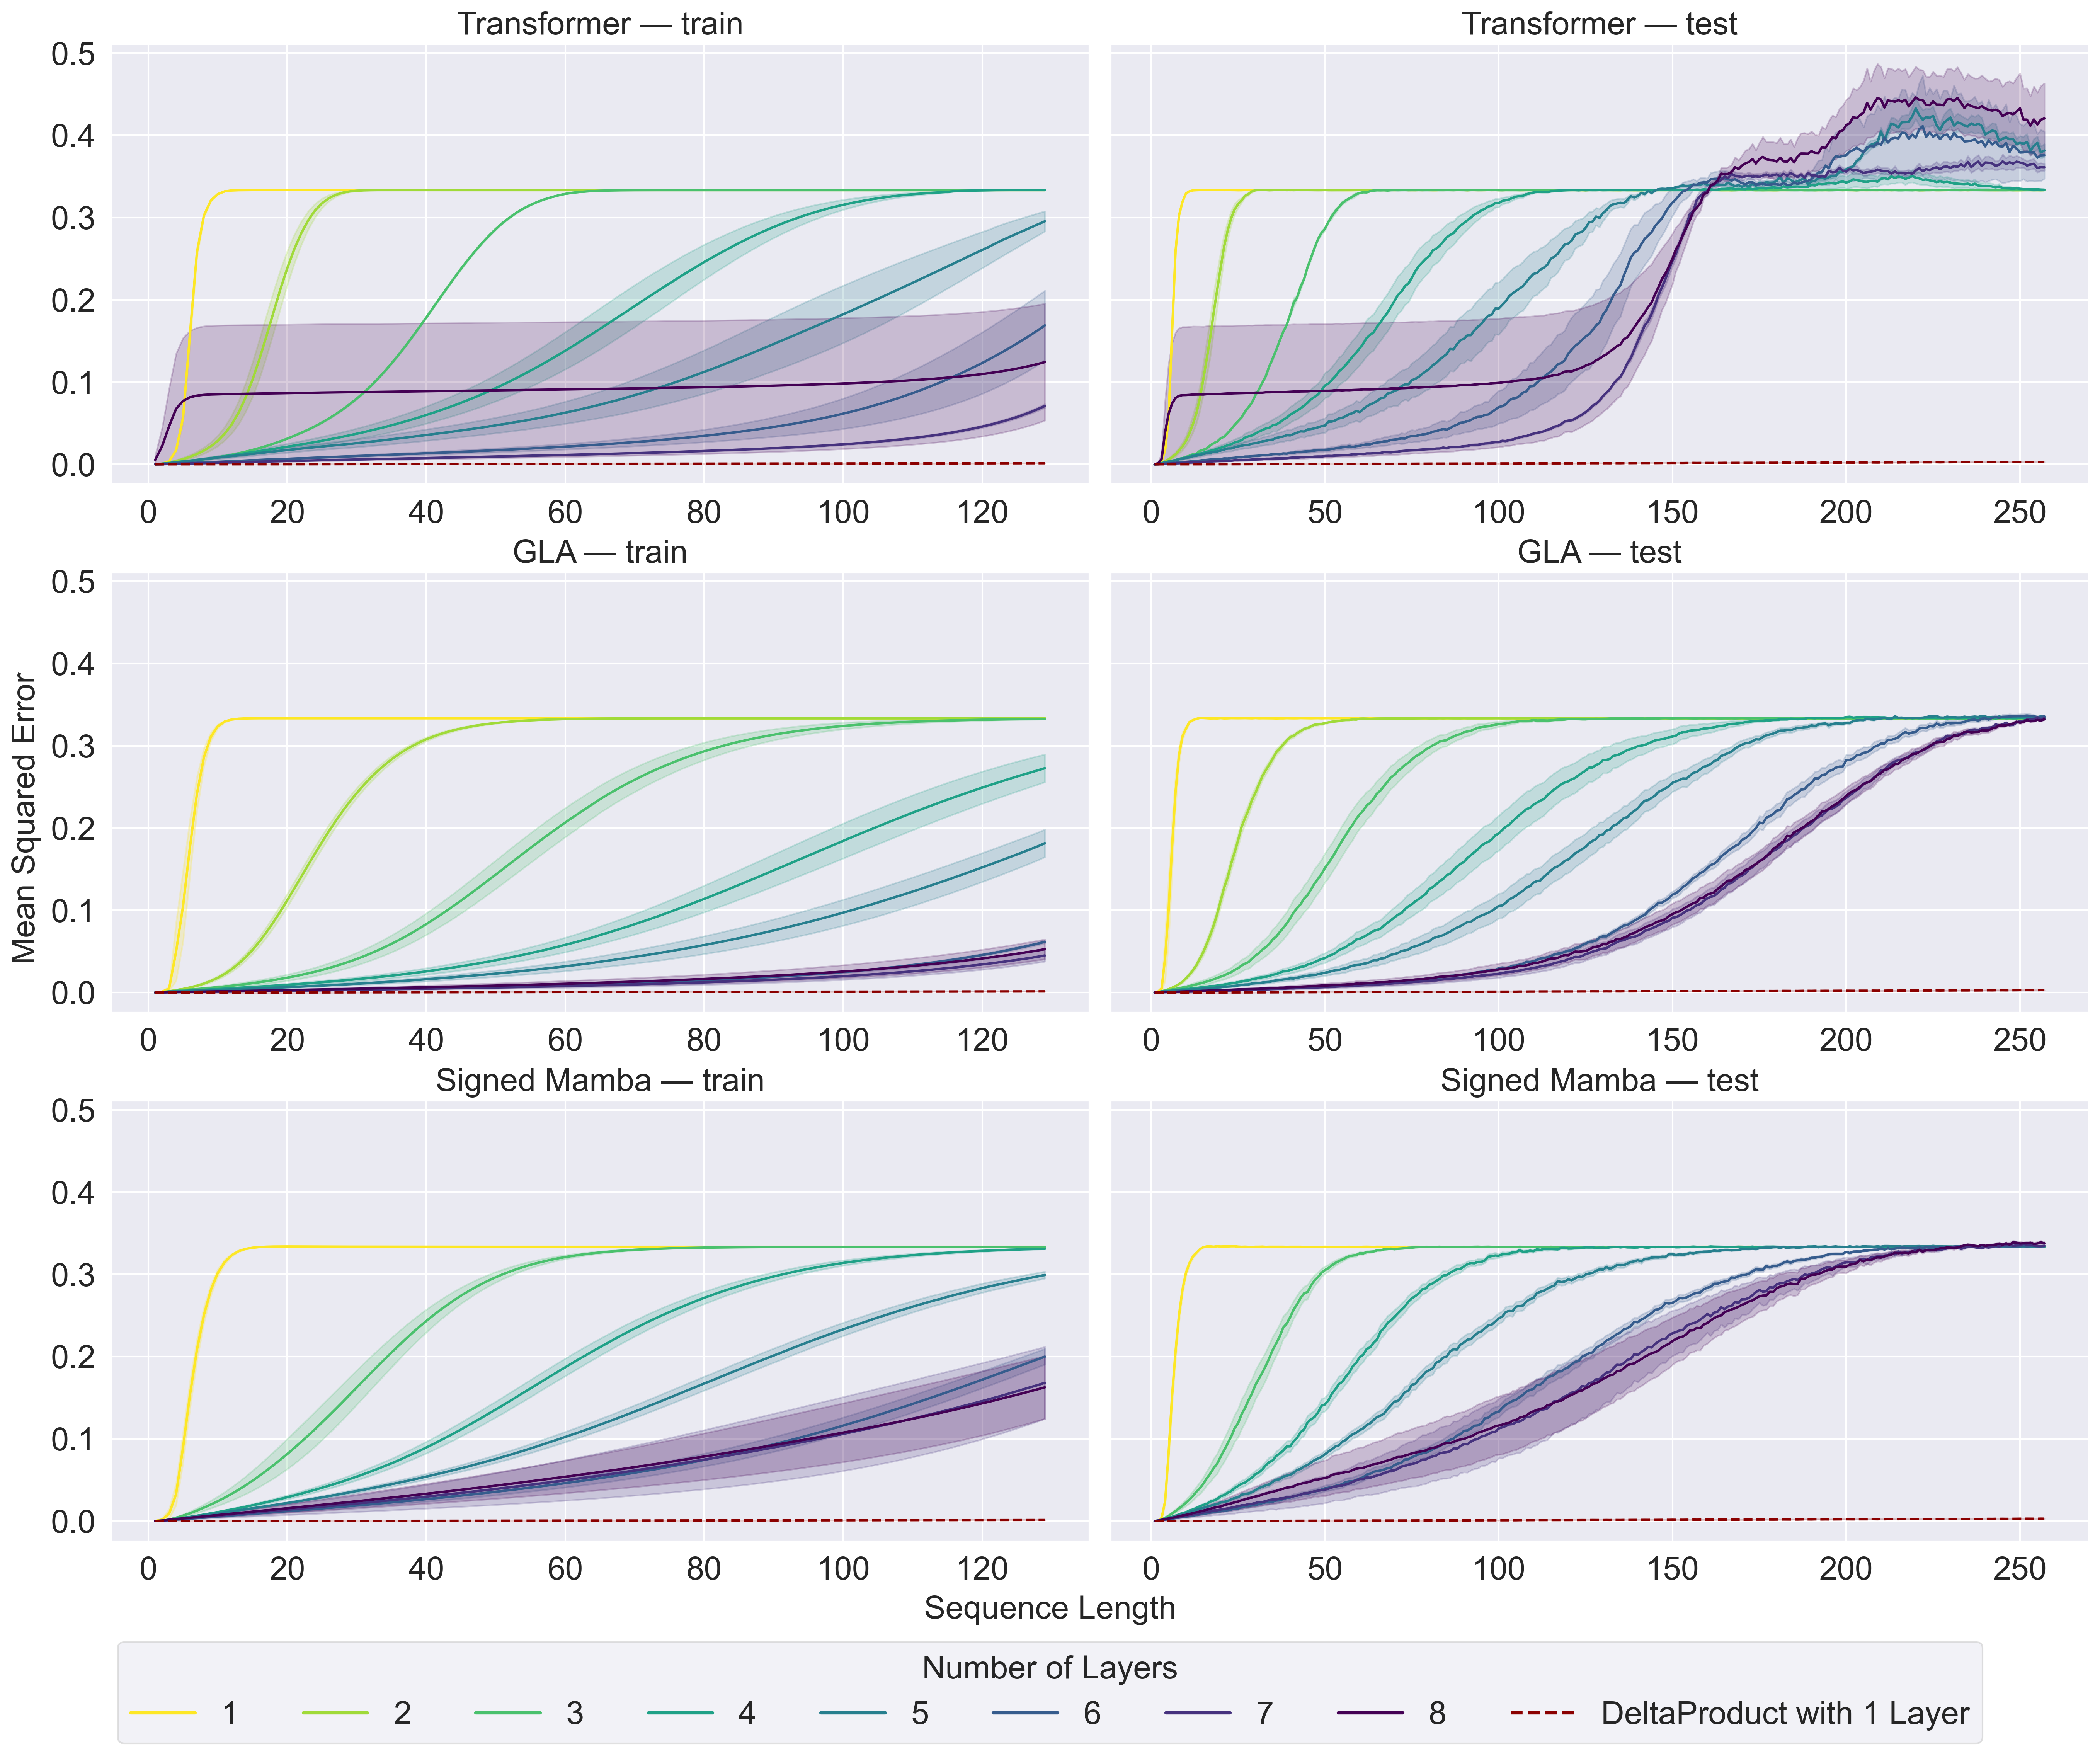
\includegraphics[width=2.0\columnwidth]{figures/mse_grid.png}
        \caption{Mean squared error on the rotated vector prediction task at various sequence length for transformer, GLA, and signed Mamba, with different numbers of layers. Left column illustrates result on training sets, and right corresponds to test sets. Standard error is shown using 3 seeds. Performance of DeltaProduct with 4 Householder products is shown as a reference.
}
        \label{fig:rotation_mse}
    \end{center}
     \vspace{-1mm}
\end{figure*}

\subsection{3D Rigid-body Rotation Problem}
\label{sec:exp_rotation}
Finally, to demonstrate the relevance of our results beyond symbolic word problems, we conduct experiments with a continuous-valued state-tracking regression problem constructed on $A_5$.

The $A_5$ group represents a symmetry on a dodecahedron.
Two chosen \emph{generators} $\{\mbf{P}, \mbf{R}\}$,
corresponding to permutation and rotation,
span $A_5$ group elements.
We represent $\{\mbf{P}, \mbf{R}\}$ in matrices:
\begin{align*}
    \mbf{P} = \begin{pmatrix}
        0 & 0 & 1 \\
        1 & 0 & 0 \\
        0 & 1 & 0
    \end{pmatrix},
    \quad
    \mbf{R} = \begin{pmatrix}
        \frac{\sqrt{5}-1}{4} & -\frac{\sqrt{5}+1}{4} & \frac{1}{2} \\
        \frac{\sqrt{5}+1}{4} & \frac{1}{2} & \frac{\sqrt{5}-1}{4} \\
        -\frac{1}{2} & \frac{\sqrt{5}-1}{4} & \frac{\sqrt{5}+1}{4}
    \end{pmatrix},
\end{align*}
where $\mbf{P}$ and $\mbf{R}$ are the permutation (or the $120^\circ$ rotation) and the $72^\circ$ rotation matrices, respectively.
We chose a vector on a unit sphere as the initial state.
The model observes a sequence of $A_5$ elements, and the task is to predict the corresponding transformed vector after each element.
Algebraically, the problem corresponds to the action of $A_5$ embedded as a finite subgroup of $SO(3,\bb{R})$. Further experimental details are provided in Appendix \ref{app:exp_rotation}.

Figure \ref{fig:rotation_mse} shows the prediction error as a function of the model depth for transformer, GLA, and Signed Mamba.\footnote{We found AUSSM to be generally unstable for this task; Appendix \ref{app:exp_rotation} provides further discussions and corresponding results.}
Analogous to the symbolic tasks, we observe that the depth plays a critical role in reducing the error.

However, here again, we observe some learnability issues for deep GLA and Signed Mamba models.
The benefit of depth on the test set performance saturates beyond 6 layers.
Similarly, the performance of deep transformer varies, illustrating a training stability issue.

\section{Discussion}
\label{sec:discussion}
The expressivity of parallelizable sequence models is limited at constant depth;
yet, deep parallelizable models achieve strong empirical performance on complex tasks.
Our work provides a Lie-algebraic perspective on this discrepancy.

Our theory connects the depth of sequence models to an abstract, algebraic extension theory.
The connection provides an optimistic message: although the algebraic obstruction may preclude an \emph{exact} simulation, deep architectures compensate to rapidly minimize the error.  This conclusion is supported by our experiments.  Across symbolic and physical tasks, we observe that increasing depth systematically reduces error on tasks outside each model's theoretical expressivity range.  Our observations suggest depth as a structural mechanism that mitigates complex order sensitivity.
This also motivates parallelizable models with adaptive depth \citep{dehghani2018universal,csordas2021devil,csordas2021ndr,csordas2024moeut,tan2023sparse}

Together, our study clarifies expressivity bounds of sequence models and how the bound is mitigated by approximation, providing a practical guideline for model selection.

\subsection{Future directions}
Our results naturally suggest several future directions.
One immediate direction is examining the impact of positional encoding (PE).
Although additive PE is unlikely to unlock expressivity,
an advanced form of multiplicative PE does boost the expressivity of commuting sequence models \cite{liu2022transformers,yang2025path}.
Understanding, or constructing, such mechanisms through algebraic structure
is a promising and practical avenue of research.

Orthogonally, our theory assumes real arithmetic and may be sensitive to the use of finite precision in real-world applications.  On the one hand, exponentially vanishing error may fall below numerical resolution, potentially blurring the algebraic obstruction. On the other hand, finite precision may constrain learnability of the system under gradient-based optimization, which we have not studied. How finite precision interacts with our findings and impacts expressivity needs to be deeply considered.

Lastly, improvements in training algorithms may improve the learnability of sequence models, allowing more extensive testing of the bounds derived here.

\subsection{Related Work}
\paragraph{Transformer variants.}
The expressivity of sequence models is often studied through computational complexity and formal language theory \citep{GilesSCLC89,gers2001lstm,schmidhuber2001evaluating,weissGY18,hahn2020theoretical,MerrillWGSSY20,BhattamishraAG20,deletang2022neural,irie2023practical,StroblMW0A24,beck2024xlstm}.
In particular, \citet{liu2022transformers} provided insight on transformer learning a semiautomaton.
By leveraging Krohn-Rhodes theorem, they guaranteed the existence of constant-depth transformer that can simulate any semiautomaton with bounded sequence length.
They further showed that no constant-depth transformer simulates general semiautomaton with arbitrary length sequence unless $\text{TC}^0 = \text{NC}^1$, and empirically showed the brittleness of the solution a transformer learns on fixed sequence length.
\citet{hu2024limitation} extended the result to (hidden) Markov model variants and empirically observed that the minimal required transformer layer depth grows logarithmically with the Markov model sequence length.
\citet{cheng2025transformers} leverage graph theory to show that a transformer can learn directed acyclic graph structures,
which can be understood as a variant of the Markov model results provided above.

\paragraph{Structured SSMs.}
\citet{merrill2024illusion} extended circuit complexity theory to SSMs and again proved constant-depth commuting SSMs, such as Mamba, are expressively limited in a way similar to constant-depth transformers. Specifically, they proved that constant-depth commuting SSMs can be simulated in $\text{TC}^0$-class circuits and thus fail to admit $\text{NC}^1$-class circuits unless $\text{TC}^0 = \text{NC}^1$.
For $S_5$ word problems, they show that the minimal required depth of Mamba or a transformer indeed grows with the sequence length.
They also proposed architectural augmentations such as nonlinear recurrence or input-dependent, non-diagonal SSMs that can, in a tradeoff with computational cost, recover expressivity with constant-depth.

Naturally, a growing body of work aims to expand SSM expressivity at tolerable computational expense.
\citet{siems2025deltaproduct} leverage input-dependent compositions of generalized Householder transformations, grounded on \citet{schlag2021linear} and \citet{yang2024parallelizing}.
They proved that (gated) DeltaProduct can theoretically recognize regular language with enough number of Householder transformation, and empirically tested with a few specific word problems.
Complementarily, another line of work leverages controlled differential equation (CDE) and rough path theory \cite{muca2024theoretical}.
Building on \citet{walker2024log},
\citet{walker2025structured} proposed structured linear CDEs (SLiCEs)
in formalizing SSMs and proved their expressivity range.
Recent work \cite{anonymous2025the} proved $L$-layer complex-valued diagonal SSMs can track solvable groups of $\le L$ derived length. They also reported the empirical demonstrated expressivity-learnability gap.
\section{Conclusion}
Scalable sequence models achieve parallelism by imposing order symmetry, which limits their ability to \emph{exactly} solve many sequence problems. We make this performance gap tangible and measurable by Lie theory and connect the depth of sequence models to algebraic extension theory. Our theory shows that, even when exact simulation is not possible, the order-sensitive approximation error vanishes exponentially with depth.
Experiments on symbolic word problems and 3D rotation state tracking task supports our theory, while also exposing practical challenges such as the instability during training of deep models. Together, we provide an algebraic perspective for understanding depth-dependent error-expressivity in parallelizable sequence models.

\section*{Impact Statement}
This paper presents work whose goal is to advance the field of Machine
Learning. There are many potential societal consequences of our work, none
which we feel must be specifically highlighted here.

\section*{Software and Data}
Our code is available at: \url{https://github.com/kazuki-irie/lie-algebra-state-tracking}.

\bibliography{main, main_2}
\bibliographystyle{icml2026}

\newpage
\appendix
\onecolumn

\section{Lie algebra for proofs}
\label{app:LieAlgebra}
In this section, we introduce further mathematical preliminaries
as necessary to provide self-contained proofs of our theorems.
We omit rigorous proofs for these observations,
and interested readers are directed to related textbooks and research papers \cite{iserles2000lie,lee2003smooth, petrogradsky2007wreath, tu2008manifold, rotman2009introduction, hall2013lie, robbin2022introduction,liu2022transformers}.
We open the section with the Lie group and Lie group action to motivate our Lie-algebraic approach.
\subsection{Lie groups and Lie algebras}
\label{app:subsubsec_Lieintro}
A set $G$ is a semigroup when $G$ is closed under an associative binary operation $\cdot: G \times G \to G$, usually called a "multiplication" operation.
If $\exists e \in G$ such that $e \cdot g = g \cdot e = g$ for $\forall g \in G$, $G$ is a monoid.
Moreover, $G$ is a group if for $\forall g \in G$ there exists an element $g^{-1} \in G$ such that $g^{-1} \cdot g = g \cdot g^{-1} = e$.
\paragraph{Lie group and Lie group action}
A Lie group $G$ is a smooth manifold equipped with a group structure under smooth multiplication.
For $x,y \in G$ let us denote the left translation $L_x(y) = xy$.
From the smoothness of the multiplication,
$L_x: G \to G$ is a diffeomorphism of the underlying manifold $\mcal{G}=G$.
In other words, translation can be thought of $G$ \emph{acting} on $\mcal{G}$.
The notion of Lie group \emph{action} generally follows:
\begin{definition}[Lie group action]
\label{app:def_LieGroupAction}
    Given a Lie group $G$ and a smooth manifold $\mcal{M}$,
    a (left) Lie group action is a smooth map
    $\Gamma: G \times \mcal{M} \to \mcal{M}$ that satisfies
    $\Gamma(e,h) = h$ and $\Gamma(xy,h) = \Gamma(x, \Gamma(y,h))$
    for an identity $e \in G$, any two elements $x, y \in G$,
    and a point on manifold $h \in \mcal{M}$.
\end{definition}
Following, we define the \emph{orbit} of $h$ denoted as $\text{Orb}_G(h) := \{\Gamma(g,h) \mid g \in G\}$.
\emph{Stabilizer}, or an isotropy subgroup, is a subgroup of $G$ where $\text{Stab}_G(h):= \{g\in G \mid \Gamma(g,h) = h \}$.

While \cref{app:def_LieGroupAction} straightforwardly describes how $\Gamma$ operates on $\mcal{M}$,
it is often advantageous to consider $\Gamma$ as inducing a diffeomorphism on $\mcal{M}$.
We can naturally introduce a Lie group homomorphism
$\Pi: G \to \text{Diff}(\mcal{M})$ such that $\Pi(g)=\Gamma(g,\cdot)$,
where $\text{Diff}(\mcal{M})$ denotes collection of diffeomorphisms of $\mcal{M}$.
\paragraph{Lie bracket and Lie algebra}
Now one may consider a smooth vector field $V: G \to TG$
and their collection $\fr{X}(G)$.
Given the differential of the left translation at point $y$,
\begin{equation*}
    (dL_x)_y: T_yG \to T_{L_x(y)}G = T_{xy}G,
\end{equation*}
the pushforward $(L_x)_*V \in \fr{X}(G)$ is well-defined \cite{tu2008manifold,lee2003smooth}.
Then, $V$ is said to be left-invariant when $(L_x)_*V = V$.
In other words, a left-invariant vector field $V$
satisfies $\bigl((L_x)_*V\bigr)_{xy} = (dL_x)_yV_y = V_{xy}$ for $\forall x, y \in G$
and completely determined by its evaluation at identity, as $V_x = V_{xe} = (dL_x)_e V_e$.
Thus, a collection of left-invariant vector fields, $\fr{X}_L(G)$, has a one-to-one correspondence with $T_e G$.

As a tangent vector is defined by how it differentiates smooth functions,
a smooth vector field on $\mcal{M}$
is commonly identified as the derivation $C^{\infty}(\mcal{M}) \to C^{\infty}(\mcal{M})$.
Following Leibniz rule,
the Lie bracket naturally arises to satisfy the derivation property \cite{tu2008manifold}.
For $f, g \in C^{\infty}(\mcal{M})$,
\begin{align*}
    XY(fg) &= X((Yf)g + fYg) \\
    &= (XYf)g + (Yf)(Xg) + (Xf)(Yg) + f(XYg) \\
    &\neq (XYf)g + f(XYg).
\end{align*}
Observe the extra term $(Yf)(Xg) + (Xf)(Yg)$ obstructs the derivation property.
One can subtract $YX(fg)$ to cancel out the extra term,
and naturally $(XY-YX)$ is again a derivation of $C^{\infty}(\mcal{M})$.
\begin{definition}[Lie bracket of vector fields]
    Given two smooth vector fields $X, Y: M \to TM$ on an open subset $M$ of a smooth manifold $\mcal{M}$,
    their Lie bracket is defined as following:
    \begin{equation}
    \label{app:eq_LieBracketDef}
        [X,Y] f = (XY - YX)f = X(Yf) - Y(Xf), \quad \forall f \in C^\infty(M).
    \end{equation}
\end{definition}
$\fr{X}_L(G)$ is closed under the Lie bracket.
Now we are ready to associate the Lie algebra $\fr{g}$ to the Lie group $G$:
\begin{definition}[Lie algebra associated to Lie group]
\label{app:LieAlgebra_Tangent}
    For a Lie group $G$, we identify the vector space of Lie algebra $\fr{g}:=T_eG$.
    For any $X \in \fr{g}$, assign a unique $X^L \in \fr{X}_L(G)$ that satisfies $X^L(y) = (dL_y)_eX$ for $y \in G$.
    We define the Lie bracket operation on $\fr{g}$ such that for $X,Y \in \fr{g}$,
    \begin{equation*}
        [X,Y] := [X^L,Y^L](e).
    \end{equation*}
    Then a map $\pi^L:\fr{g} \to \fr{X}_L(G)$, $\pi^L(X) = X^L$ is a Lie algebra isomorphism.
\end{definition}
Naturally, Lie algebra $\fr{g}$ can also be identified as a collection of the left-invariant, first-order differential operators on $G$.
Note the Lie bracket operation depends on the identification: with $\fr{g} \cong T_eG$, $[X,Y] \in T_eG$.
On the other hand, identifying $\fr{g} \cong \fr{X}_L(G)$ produces $[X,Y] \in \fr{X}_LG$.
The identification should be clear from the context.

We can analogously define the right translation on Lie group $R_x(y) = yx$.
The differential of the right translation at point y gives $(dR_x)_y: T_yG \to T_{R_x(y)}G = T_{yx}G$,
and we denote the collection of right-invariant vector fields as $\fr{X}_R(G)$.
Notationally, one can prove that $[X^L, Y^L](e) = -[X^R, Y^R](e)$ \cite{lee2003smooth}.
In that, $\pi^R: \fr{g} \to \fr{X}_RG$, $\pi^R(X) = X^R$ swaps the Lie bracket sign.

\paragraph{Bridge to geometry}
As a concrete example, consider the open set $M$ in \cref{app:eq_LieBracketDef} with local coordinate charts $x=(x^1, \cdots, x^n)$
around point $p \in M$.
Then we can rewrite $X \in \fr{X}(M)$ in a coordinate expression:
\begin{equation*}
    X = \sum_{a=1}^n X^a \partial_a,
    \quad
    X^a = X(x^a) \in C^\infty(M),
\end{equation*}
and similarly for $Y \in \fr{X}(M)$.
Given the local coordinate, Lie brackets get a tangible interpretation.
One can exhaust the vector field Lie brackets with coordinate,
\begin{align*}
    [X,Y] = \sum_{c=1}^n [X,Y]^c \partial_c,
    \quad
    [X,Y]^c = X(Y^c) - Y(X^c),
\end{align*}
where $[X,Y]^c$ is again a coordinate function of $[X,Y] \in \fr{X}(M)$.
Evaluated at $p$, $[X,Y]^c(p) = X_p(Y^c) - Y_p(X^c)$.
Then from the differential it is transparent:
\begin{equation}
\label{app:eq_LieBracket_Directional}
    [X,Y]^c(p) = X_p(Y^c) - Y_p(X^c) = (dY^c)_p(X_p) - (dX^c)_p(Y_p).
\end{equation}
One may interpret above as a directional derivative of a smooth coordinate function
along the tangent vector direction \cite{lee2003smooth}.

\subsection{Representation and infinitesimal action}
\label{app:subsubsec_repprelim}
\paragraph{Lie group representation}
The abstract notion provided at \cref{app:subsubsec_Lieintro} is often easier to work with a tangible object,
and matrix is one of such.
As $g, g^{-1} \in G$, let us consider the collection of any invertible matrices in $\bb{R}^{n \times n}$.
Over the real field, we name the collection as the general linear group and denotes as $\G{GL}{n;\bb{R}}$.
Matrix Lie group is defined as a closed subgroup of $\G{GL}{n;\bb{R}}$,
and many Lie groups in application arise as one.

These are the case of \emph{Lie group representations} \cite{lee2003smooth, hall2013lie}.
Given a real vector space $V$,
a representation of Lie group $G$ is a Lie group homomorphism $\Pi: G \to \G{GL}{V}$.
When $\dim V = n$, we can identify $\G{GL}{V}$ with $\G{GL}{n;\bb{R}}$ via basis choice.
Recall \cref{app:def_LieGroupAction} that representation is just a linear Lie group action of $G$ on $V$.
\paragraph{Lie algebra representation}
With \cref{app:LieAlgebra_Tangent} we can think of the corresponding \emph{Lie algebra representations}.
For a Lie group $G$ associated with $\fr{g}$,
consider $X \in \fr{g} \cong T_eG$ and corresponding $X^L \in \fr{X}_L(G)$.
Let $c_X: \bb{R} \to G$ be the integral curve of $X^L$ with $c_X(0) = e \in G$, starting at the identity.
Then we can construct the exponential map,
which is a canonical smooth map from the Lie algebra to its integrating group \cite{lee2003smooth}:
\begin{equation*}
    \exp: \fr{g} \to G, \quad \exp(X):= c_X(1),
\end{equation*}
and we write $\exp(tX) = c_X(t)$ so that $\frac{d}{dt}\vert_{t=0} \exp(tX) = X$.
Notice that $X$ corresponds to the initial velocity of $c_X(t)$.

One concrete example is the matrix Lie algebra $\fr{gl}(n,\bb{R})$, which is a collection of any matrices in $\bb{R}^{n \times n}$.
With the Lie group representation:
\begin{equation*}
    \Pi: G \to \G{GL}{n;\bb{R}}, \quad \Pi_*: T_eG \to T_{\Pi(e)}\G{GL}{n;\bb{R}} = T_{I_n}\G{GL}{n;\bb{R}},
\end{equation*}
where we identified $\G{GL}{n;\bb{R}}$-associated Lie algebra
$\fr{gl}(n,\bb{R}) \cong T_{I_n}\G{GL}{n;\bb{R}}$.
Then the Lie algebra representation is naturally induced:
\begin{equation*}
    \pi:= (d \Pi)_e: \fr{g} \to \fr{gl}(n,\bb{R}),
\end{equation*}
in that, $\pi$ is the differential of $\Pi$ at the identity.
For the matrix Lie algebra, exponential map is the matrix exponential $\text{expm}$:
\begin{equation}
\label{app:eq_matrixLie_exponential_action}
    \Pi(\exp(X)) = \text{expm} (\pi(X)), \: \pi(X) = \frac{d}{dt}\bigg\vert_{t=0}\Pi(\exp(tX)).
\end{equation}
We extend the differential of representation to the differential of action,
or \emph{infinitesimal} action, in the following paragraph.
\paragraph{Fundamental vector field}
Consider the Lie group $G$ acts on itself by left multiplication.
For $h \in G$ and $X \in \fr{g}$, let us define a vector field $X^\sharp$:
\begin{equation*}
    X^\sharp(h) = \frac{d}{dt} \bigg \vert_{t=0} \exp(-tX)h = -(dR_h)_eX \in T_hG.
\end{equation*}
Observe that $X^\sharp(h)$ recovers familiar ODE $\dot{h} = Xh$
up to sign change, when $G \subseteq \G{GL}{n,\bb{R}}$.

We can extend above to an arbitrary smooth finite manifold $\mcal{M}$,
replacing canonical left action on $G$ to a chosen left Lie group action $\Gamma: G \times \mcal{M} \to \mcal{M}$.
For each $X \in \fr{g}$ and $h \in \mcal{M}$, we define the fundamental vector field $X^\sharp \in \fr{X}(\mcal{M})$:
\begin{equation}
\label{app:eq_fundamental_vector_field}
    X^\sharp (h) := \frac{d}{dt}\bigg\vert_{t=0}\Gamma(\exp(-tX), h) \in T_h\mcal{M},
\end{equation}
then the map $\gamma: \fr{g} \to \fr{X}(\mcal{M})$,
$\gamma(X)= X^\sharp$ is a Lie algebra homomorphism \cite{iserles2000lie, robbin2022introduction}.
Therefore $\gamma$ is an \emph{infinitesimal} Lie group action, and considered as Lie algebra action on $\mcal{M}$.
\begin{remark}
\label{app:rem_Bracket_Sign}
Many text writes $X^\sharp$ in a \emph{right-invariant} vector field form \cite{robbin2022introduction}:
\begin{equation}
\label{app:eq_fundamental_vector_field2}
    X^\sharp (h) := \frac{d}{dt}\bigg\vert_{t=0}\Gamma(\exp(tX), h) \in T_h\mcal{M},
\end{equation}
and the map $\gamma(X)= X^\sharp$ is a Lie algebra \emph{anti}homomorphism \cite{iserles2000lie, robbin2022introduction}.
Under this definition, one would observe that $[\pi(X), \pi(Y)] = \pi([X,Y])$, a matrix commutator,
aligns with $[X^\sharp, Y^\sharp] = -[X,Y]^\sharp$ up to sign change.
In practice, the sign can be absorbed and need not be worried.
Some literature swap the Lie bracket direction to handle the sign change,
but this is just a choice of convention and does not obstruct any fundamental logic.
\end{remark}
\paragraph{Bridge to homogeneous ODE}
\label{app:bridge_to_hom_LPV}
As observed above, when a Lie group $G \subseteq \G{GL}{n,\bb{R}}$ left-acts on a smooth manifold $\mcal{M} \cong \bb{R}^n$,
the fundamental vector field recovers homogeneous ODE.
For a point $h \in \mcal{M}$ and $\mbf{A} \in \fr{g} \subseteq \fr{gl}(n,\bb{R})$, we select $\Gamma$ to be a left multiplication.
Then obviously:
\begin{equation*}
    \dot{h} = \frac{d}{ds}\bigg\vert_{s=0}\Gamma(\exp(s\mbf{A}), h) = \mbf{A}h,
\end{equation*}
which corresponds to the linear controlled homogeneous ODE, $\dot{h}(t) = \mbf{A}(x(t))h(t)$, given a fixed input $x(t)$.

Critically, when $G$ acts on itself, we can recover the state-transition matrix $\Phi$.
Recall \cref{def:Phi}, $\Phi$ satisfies:
\begin{equation}
\label{app:eq_homogeneous_matrix_state}
    \dot{\Phi}(t,0) = \mbf{A}(x(t))\Phi(t,0), \quad \Phi(0,0) = I_n,
\end{equation}
then \cref{app:eq_homogeneous_matrix_state} forms a homogeneous ODE system with $\Phi$ being its latent state.
This observation is very useful:
it is immediate that for any admissible input, $\Phi(t,0) \in G$.
In a sense, one may understand \cref{app:eq_homogeneous_matrix_state}
as tracking \emph{every} possible state evolution, rather than a single state.
This is a conventional perspective in geometric control theory,
commonly referred as control theory on Lie groups \cite{jurdjevic1972control, iserles2008magnus}.

\subsection{Lie algebra extension}
\label{app:subsubsec_extensionprelim}
Analogous to the notion of the group extension, Lie algebra extension formalizes \emph{gluing} two Lie algebras together.
Here we introduce the notion of Lie algebra extension \cite{weibel1994introduction,rotman2009introduction, PhysicsExtension, beckett2022symplectic}.
\begin{definition}[Lie algebra extension]
    \label{app:def_LieAlgebraExtension}
    The Lie algebra $\tilde{\fr{h}}$ is an extension of base Lie algebra $\fr{h}$ by (finite-dimensional) kernel Lie algebra $\fr{a}$ if there exists a short exact sequence of Lie algebras:
    \begin{equation}
    \label{app:eq_LieAlgebraExtension_shortsequence}
        0 \to \mathfrak{a} \xrightarrow{i} \tilde{\mathfrak{h}} \xrightarrow{\theta} \mathfrak{h} \to 0.
    \end{equation}
\end{definition}
Redundantly, $i: \fr{a} \to \tilde{\fr{h}}$ is a Lie algebra monomorphism,
while $\theta: \tilde{\fr{h}} \to \fr{h}$ is a Lie algebra epimorphism.
The short exact sequence satisfies $\text{im}\; i = \ker \theta$,
thus $i(\fr{a})$ is an ideal in $\tilde{\fr{h}}$ and $\tilde{\fr{h}}/i(\fr{a}) \cong \fr{h}$.
Following common convention, we identify $\fr{a}$ with $i(\fr{a})$ without confusion.
\begin{remark}[Tower of abelian extension]
\label{app:rem_solvable_k_tower}
A solvable Lie algebra with derived series $\fr{g} = \fr{g}^{(0)} \supset \fr{g}^{(1)} \supset \cdots \supset \fr{g}^{(k)}=\{0\}$
is an extension:
\begin{equation*}
    0 \to \fr{g}^{(n)} \to \fr{g} \to \fr{g} / \fr{g}^{(n)} \to 0.
\end{equation*}
When $n = k-1$, $\fr{g}^{(k-1)}$ is an abelian Lie (sub-)algebra and
$\fr{g} / \fr{g}^{(k-1)}$ is a solvable Lie algebra of derived length $k-1$.
In iteration, we recover a $k$-length \emph{tower} of abelian Lie algebra extension.
\paragraph{Split extension}
Understanding how $\fr{h}$ acts on $\fr{a}$ is critical in characterizing $\tilde{\fr{h}}$.
We begin with a simple case.
\end{remark}
\begin{definition}[Split extension]
    In \cref{app:eq_LieAlgebraExtension_shortsequence}
    consider a linear section $s: \fr{h} \to \tilde{\fr{h}}$ that satisfies $\theta \circ s = 1_\fr{h}$, an identity map.
    If $s$ is a Lie algebra homomorphism, \cref{app:eq_LieAlgebraExtension_shortsequence} is \emph{split}.
\end{definition}
If Lie algebra extension splits, then
we say $\tilde{\fr{h}}$ is a \emph{semidirect product} (or sum) of $\fr{h}$ by $\fr{a}$
and we denote as $\tilde{\fr{h}} = \fr{h} \ltimes \fr{a}$
(or $\fr{a} \rtimes \fr{h}$) \cite{rotman2009introduction}.\footnote{Note
that the convention of sign direction is not accordant across references \cite{petrogradsky2007wreath, rotman2009introduction}.
here we emphasize that $\fr{h}$ acts on $\fr{a}$.}

Consider $X,Y \in \fr{h}$ and $u,v \in \fr{a}$.
$\tilde{\fr{h}}$ acts on $\fr{a}$ by derivation, as $\fr{a}$ is an ideal in $\tilde{\fr{h}}$.
As the linear section $s$ is a Lie algebra homomorphism,
$s(X) \in \tilde{\fr{h}}$ naturally acts on $\fr{a}$ by derivation too.
Thus, the induced action of $\fr{h}$ on $\fr{a}$ is straightforward here:
\begin{equation*}
    \rho: \fr{h} \to \text{Der}(\fr{a}),
    \quad
    \rho(X)v = [s(X),v],
\end{equation*}
and Lie bracket on split extension follows:
\begin{align}
\label{app:eq_split_bracket}
    [(X, u), (Y, v)]_{\tilde{\fr{h}}} &= ([X,Y]_\fr{h}, [u,v]_\fr{a} + \rho(X)v - \rho(Y)u).
\end{align}
One special case of split extension is the trivial extension where $[(X,u),(Y,v)] = ([X,Y],[u,v])$,
and we name it as a \emph{direct product} (or sum) of $\fr{h}$ and $\fr{a}$.

\paragraph{Bridge to inhomogeneous ODE}
\label{app:bridge_to_general_LPV}
Similar to \cref{app:bridge_to_hom_LPV}, affine vector field naturally arises from the semidirect product.
Consider an inhomogeneous ODE $\dot{h}(t) = \mbf{A}(x(t))h(t) + \mbf{b}(x(t))$.
As noted often \cite{krener1975bilinear, krener1977decomposition, iserles2000lie},
one can augment the state to \emph{homogenize} the ODE:
\begin{equation*}
    \bar{h}(t) = \begin{pmatrix}
    h(t) \\
    1
\end{pmatrix},
\quad
\dot{\bar{h}}(t)
= \begin{pmatrix}
        \mbf{A}(x(t)) & \mbf{b}(x(t)) \\
        0 & 0
    \end{pmatrix}
    \:
    \bar{h}(t).
\end{equation*}
Then it is immediate that the generator class is affine.
Consider a finite-dimensional Lie group of affine transformation, $\G{Aff}{n, \bb{R}}$.
Its associated Lie algebra $\fr{aff}(n, \bb{R})$ is the canonical example of the split extension:
\begin{equation*}
    0 \to \bb{R}^n \to \fr{aff}(n, \bb{R}) \to \fr{gl}(n,\bb{R}) \to 0,
\end{equation*}
such that $(A,b) \in \fr{gl}(n,\bb{R}) \ltimes \bb{R}^n$.
With a standard matrix embedding,
\begin{equation*}
    (A,b) \longmapsto \begin{pmatrix}
        A & b \\
        0 & 0
    \end{pmatrix},
\end{equation*}
which corresponds to the generator class of the homogenized ODE above.

Let us confirm that realized SSM respects the split extension bracket rule in \cref{app:eq_split_bracket}.
From the matrix representation above, one can simply check their matrix commutator.
With two fixed inputs $x$, $y$:
\begin{equation*}
    \bar{\mbf{A}}(x) = \begin{pmatrix}
        \mbf{A}(x) & \mbf{b}(x) \\
        0 & 0
    \end{pmatrix},
    \quad
    [\bar{\mbf{A}}(x), \bar{\mbf{A}}(y)]
    =
    \begin{pmatrix}
        [\mbf{A}(x), \mbf{A}(y)]
        &
        \mbf{A}(x)\mbf{b}(y) - \mbf{A}(y)\mbf{b}(x) \\
        0 & 0
    \end{pmatrix},
\end{equation*}
especially when $\text{Lie}{\{\mbf{A}(x)\}}$ is abelian, $[\mbf{A}(x), \mbf{A}(y)] = 0$ and only the top right entry is nonzero.

Now consider vector field representation. For the brevity, let us keep $\text{Lie}{\{\mbf{A}(x)\}}$ be abelian.
Recall \cref{app:eq_LieBracket_Directional}:
\begin{align}
X(h) &= \mbf{A}(x)h + \mbf{b}(x), \quad Y(h) = \mbf{A}(y)h + \mbf{b}(y) \nonumber \\
    [X,Y]^c &= \sum_{a=1}^{n}
    \left(
    \mbf{b}^a(x)\mbf{A}^{ca}(y)
    - \mbf{b}^a(y)\mbf{A}^{ca}(x)
    \right) \nonumber \\ 
    [X,Y] &= \mbf{A}(y)\mbf{b}(x) - \mbf{A}(x)\mbf{b}(y),\label{app:eq_LPV_affinebracket}
\end{align}
with sign change noted in \cref{app:rem_Bracket_Sign}.

Taken together with \cref{app:bridge_to_hom_LPV},
switching the vector state space
with the corresponding Lie group, or flow space,
is often referred as \emph{lifting} \cite{krener1977decomposition}.
Except for minor details in implementation, lifting does not lose any generality
and we can \emph{project} back to the state space \cite{iserles2000lie, iserles2008magnus}.
\paragraph{Central extension and beyond}
If all extension belongs to the split extension class, our discussion would be much easier.
However note that the linear section $s: \fr{h} \to \tilde{\fr{h}}$ needs not be a Lie algebra homomorphism.
Among non-split extension, central extension is another key class of the Lie algebra extension.
\begin{definition}[Central extension]
    In \cref{app:eq_LieAlgebraExtension_shortsequence} let $\fr{a}$ be abelian.
    When $i(\fr{a})$ is in the center of $\tilde{\fr{h}}$ such that $[\tilde{X}, u] = 0$ for any $\tilde{X} \in \tilde{\fr{h}}$
    and $u \in i(\fr{a})$, we call it as central extension.
\end{definition}
As $s$ is not necessarily Lie algebra homomorphism, we introduce a correction term, called \emph{2-cocycle} \cite{weibel1994introduction}:
\begin{equation}
\label{app:eq_2cocycle}
    \omega: \fr{h} \times \fr{h} \to \fr{a}, \quad
    \omega(X,Y) := [s(X),s(Y)] - s([X,Y]_\fr{h}).
\end{equation}
Recall \cref{app:eq_split_bracket}.
As $\fr{a}$ belongs to the center, the induced action $\rho: \fr{h} \to \text{Der}(\fr{a})$ is trivial.
Thus, in central extension, the bracket rule simplifies to:
\begin{equation*}
\label{app:eq_central_bracket}
[(X,u),(Y,v)] = ([X,Y], \omega(X,Y)).
\end{equation*}
When $s$ is Lie algebra homomorphism, central extension breaks down to trivial extension.

Taken together, the Lie bracket on general Lie algebra extension follows:
\begin{equation*}
    [(X, u), (Y, v)]_{\tilde{\fr{h}}} = [[X,Y]_\fr{h}, [u,v]_\fr{a} + \rho(X)v - \rho(Y)u + \omega(X,Y)].
\end{equation*}
Characterization of general Lie algebra extension is nontrivial.
At least under Lie group setting, the Kaloujnine-Krasner universal embedding theorem states that
any Lie group extensions embeds into the \emph{wreath} product of Lie group \cite{wells1976some,deval2024universal}.
Fortunately, following studies have extended the universal embedding theorem
to Lie algebra \cite{petrogradsky2007wreath, deval2024universal}.
\section{Control theory basics}
\label{app:LPV}
\subsection{Abstract control systems}
\label{app:control_detail}
Here we discuss abstract notions of controlled dynamical systems \cite{iserles2000lie}.
On a real smooth finite-dimensional manifold $\mcal{M}$, we consider a time-dependent tangent vector field:
\begin{equation*}
    F: [0,\tau] \times \mcal{M} \times \mcal{X} \to T\mcal{M},
\end{equation*}
which is locally Lipschitz in $h \in \mcal{M}$ and measurable in time $t \in [0,\tau]$.  
In this context, we call $\mcal{M}$ the \emph{state space} and $\mcal{X}$ the \emph{input space}.
Then, with a fixed input path $x: [0,T] \to \mcal{X}$ we obtain the controlled ODE:
\begin{equation}
    \label{eq:abstractODE}
    \dot{h}(t) = F_x(t,h(t)), \; F_x(t,h(t)) := F(t,h(t),x(t)),
\end{equation}
assuming the path is locally bounded and integrable \cite{iserles2000lie}.
We call a tuple $S = (\mcal{M}, F,\mcal{X})$ a \emph{controlled dynamical system}.
Lastly, we say the system is initialized when $h(0)$ is fixed.
Restricting $\mcal{M}$ to be on a Euclidean state space realizes SSM.
\subsection{Simulation}
\label{app:sim_detail}
Here we formally introduce the notion of simulation \cite{sussmann1976existence,hermann1977nonlinear, krener1977decomposition}.
\begin{definition}[Simulation]
\label{def:SSM_sim_equivalence}
    Let two initialized $S_0$, $S_1$ share an input space.
    Consider a smooth map $\varphi: \mcal{M}_0 \to \mcal{M}_1$
    such that $\varphi(h_0(t)) = h_1(t)$ for any admissible inputs.
    If $\varphi$ is a surjective submersion, we say $S_0$ \emph{simulates} $S_1$.
    Moreover, if $\varphi$ is (locally) diffeomorphic, we say $S_0$ is equivalent to $S_1$.
\end{definition}
Note that if $S_0$ simulates $S_1$ and $\dim S_0 = \dim S_0$,
then $\varphi$ is diffeomorphic.
Therefore, equivalence implies simulation.

For SSMs, $\varphi$ is restricted to be full-rank linear map.
Following, diffeomorphic $\varphi$ is invertible linear map.
Arbitrary smooth $\varphi$ would typically leave the SSM model class \cite{krener1977decomposition,toth2010modeling}.
When restricted to SSMs, we define simulation error correspondingly.
\begin{definition}[SSM Simulation error on horizon]
\label{def:SSM_sim_error}
    Consider initialized $\mbf{S}_0$, $\mbf{S}_1$ with $n_0 = \dim \mbf{S}_0 \ge \dim \mbf{S}_1 = n_1$.
    Let $\mcal{X}_{ad}$ be shared admissible input path space, with
    \begin{equation*}
        U := \{x \in \mcal{X}_{ad} \mid x: [0,T] \to \mcal{X}, \|x\| \le M\}
    \end{equation*}
    be measure bounded paths over chosen interval $[0,T]$.
    Then, we define simulation error:
    \begin{equation}
    \label{eq:SSM_sim_error}
    \Delta_h := \inf_{\mbf{P} \in \bb{R}^{n_1 \times n_0}} \sup_{x \in U} \bigl\| \mbf{P}h_0(T) - h_1(T) \bigr\|,
    \end{equation}
    where $\mbf{P}$ is a full-rank linear map.
\end{definition}
Note that $\mbf{P}$ can be replaced with invertible linear map $\mbf{T}$
by state augmentation on $\mbf{S}_1$, which leads to the standard state-space equivalence relation
in linear parameter-varying (LPV) system theory \cite{toth2010modeling}.
\subsection{Minimality}
\label{app:min_detail}
To understand whether one system simulates the other, we need a notion of minimality.
With a concept of Lie group action, minimality comes in a straightforward manner \cite{jurdjevic1972control, krener1977decomposition}.

Consider $5$-tuple $(\mcal{M},F,\mcal{X}_{ad},\mcal{Y},g)$
and its evolution operator $\Psi$.
Consider a collection $S = \{\Psi_x\}$ for $x \in \mcal{X}_{ad}$,
then one can notice $S \subset \text{Diff}(\mcal{M})$ is a semigroup.
Although any $\Psi_x(t,0)$ represent as an invertible matrix,
the existence of admissible input for $\Psi_{x'} = \Psi_x^{-1}$ is not guaranteed.
With completion, we denote a group $G$ be the smallest subgroup of $\text{Diff}(\mcal{M})$ containing $S$.

For a chosen point $h \in \mcal{M}$, consider a collection $S(h) = \{\Psi(h): \Psi \in S\}$ and $G(h) = \{\Psi(h): \Psi \in G\}$.
It is akin to the orbit of Lie group action:
intuitively, $S(h)$ is the set of accessible points on $\mcal{M}$ under admissible inputs.
We say the system is (weakly) \emph{controllable} at point $h$ when $S(h) = \mcal{M}$.
When satisfied, the condition implies $G(h) = \mcal{M}$.

Now consider the output map.
Given any two points $h_1, h_2 \in \mcal{M}$, denote $y_1(t) = g(\Psi(t,0)(h_1))$ and $y_2(t)$ correspondingly.
Then $h_1$ and $h_2$ are said to be indistinguishable when $y_1(t) = y_2(t)$ for any admissible inputs.
The system is \emph{observable} when $h_1$ and $h_2$ being indistinguishable implies $h_1 = h_2$.
Collectively, we say the system $(\mcal{M},F,\mcal{X}_{ad},\mcal{Y},g)$ is \emph{minimal}
when both (weakly) controllable and observable \cite{krener1977decomposition}.
\begin{remark}
    Often, the attention is restricted to open subset $U \subseteq \mcal{M}$ however small.
    Without global Lie group action and orbits, one can characterize the system with Lie algebras.
    For example, weak controllability is replaced by \emph{Lie algebra accessibility rank condition} \cite{sontag2013mathematical}.
\end{remark}
One may easily notice the notion of minimality in LTI system is a special case of the above.
We can similarly induce notion of minimality for SSMs,
commonly studied as a (quasi-)LPV system \cite{toth2010modeling}.
\subsection{Magnus series and path signature}
\label{app:CDE}
The Magnus series provides Lie-algebraic expansion of the state-transition matrix.
As various evolution operators in physical applications are indeed a integral curve on a Lie group,
the Magnus expansion (or its truncation) serves as a useful tool in numerical approximation problems \cite{iserles2000lie}.
Given a system $\mbf{S}$, we explicitly write down a few first terms:
\begin{align*}
    \Phi(t,0) &= \exp \Omega(t),
    \quad
    \Omega(t) = \sum \Omega_i(t)\\
    \Omega_1(t) &= \int_0^t \mbf{A}(t_1) \; dt_1 \\
    \Omega_2(t) &= \frac{1}{2}\int_0^t \; dt_1 \int_0^{t_1} \; dt_2
    [\mbf{A}(t_1), \mbf{A}(t_2)] \\
    \Omega_3(t) &= \frac{1}{6}\int_0^t \; dt_1 \int_0^{t_1} \; dt_2 \int_0^{t_2} \; dt_3
    \Bigl(
    [\mbf{A}(t_1), [\mbf{A}(t_2), \mbf{A}(t_3)]] + [\mbf{A}(t_3), [\mbf{A}(t_2), \mbf{A}(t_1)]]
    \Bigr)
    \\
    \cdots
\end{align*}
Observe how the lower central series contributes to each order of the Magnus series.
Specifically, the $i$-th order Magnus term involves a linear combination of elements in the $(i-1)$-th member of the lower central series, $\fr{g}^{i-1}$.
Consequently, if $\fr{g}$ is a class $c$ nilpotent Lie algebra, then the Magnus expansion of $\mbf{S}_\fr{g}$ truncates at order $c$. As a special case, abelian $\fr{g}$ is the class $1$ nilpotent Lie algebra, all commutators of $\mbf{S}_\fr{g}$ vanish and we have truncation at order $1$.

Recent progress in continuous-time neural network modeling leverages
rough path theory and path signature \cite{muca2024theoretical, walker2024log, walker2025structured}.
Path signature is deeply related to the Magnus series \cite{chevyrev2024multiplicative,chevyrev2025primer}.
For linear CDE, the path signature can be expressed as
a tensor exponential of the Magnus expansion \cite{friz2022unified}.
In other words, the Magnus expansion is a representation of \emph{log-signature} \cite{morrill2021neural, walker2024log}
when input variation is bounded.
Log-signature underscores the algebraic property of input path,
while the Magnus expansion prioritizes state transition.
The study of the Magnus series is relatively mature and often provides both theoretical and computational benefits
when the path signature admits the Magnus expansion \cite{friz2022unified}.
\section{Proofs}
\label{app:proof}
\subsection{Proof of \cref{lem:sim_impossible}}
\label{app:sim_impossible_proof}
\begin{proof}
    Algebraically, it is straightforward.
    Any image of abelian Lie algebra under Lie algebra homomorphism is abelian.
    There is no representation of abelian Lie algebra that depends on path order.
    
    Constructively, general SSM $\mbf{S}$ and abelian SSM $\hbf{S}$ are linear ODEs.
    It suffices to find the existence of nonsingular linear state transformation map $\mbf{T}$
    that satisfies $\mbf{T}\hat{h}(t) = h(t)$ for any time $t$ and admissible inputs
    (\cref{par:sim_min_main} and \cref{app:sim_detail}).

    Let us denote $(\Phi, \hat{\Phi})$ be the state-transition matrix of $(\mbf{S}, \hbf{S})$.
    It is clear that $\mbf{T}\hat{h}(t) = h(t)$ implies $\mbf{T}\hat{\Phi}(t,0) = \Phi(t,0)\mbf{T}$.
    Consider an admissible input path $x: [0,T] \to \mcal{X}$,
    and its measure-preserving permutation path $x'(t)= x(\sigma(t))$
    where $\sigma:[0,T] \to [0,T]$.
    Assume $x'$ is also admissible.
    Then, being abelian:
    \begin{equation*}
        \hat{\Phi}_{x}(T,0) = \hat{\Phi}_{x'}(T,0),
        \quad
        \mbf{T}(\hat{\Phi}_{x}-\hat{\Phi}_{x'})\mbf{T}^{-1} = \mbf{0}.
    \end{equation*}
    However, for non-abelian $\mbf{S}$, chronological exponential map depends on the path order and $\Phi_{x}(T,0) \neq \Phi_{x'}(T,0)$,
    contradicting the existence of $\mbf{T}$.
    
    As noted in \cref{app:sim_detail}, the proof generalizes to the case $m = \dim \hbf{S} \ge \dim \mbf{S} = n$.
    $\mbf{T}$ simply needs to satisfy:
    \begin{equation*}
        \mbf{T}\hat{h} = \begin{bmatrix}
            h \\
            *
        \end{bmatrix}
        \begin{matrix*}[l]
            \rbrace \; n \\
            \rbrace \; m-n,
        \end{matrix*}
    \end{equation*}
    for some variables $*$ to match dimension \cite{toth2010modeling}.
    The algebraic nature is intact, and the proof immediately follows.
    With respect to \cref{eq:SSM_sim_error},
    truncating $*$-corresponding rows of $\mbf{T}$ recover full-rank matrix $\mbf{P}$.
\end{proof}
\subsection{Proof of \cref{thm:sim_error}}
\label{app:sim_error_proof}
Here we divide the problem into abelian and restricted cases.
Notation follows \cref{app:sim_impossible_proof}.
\begin{proof}[Abelian SSM]
    Consider general SSM $\mbf{S}$.
    Assume an input path $x$ and permuted $x'$ on window $[0,T]$ are both admissible.
    With small enough $T$, we can derive a loose lower bound of $\|\Phi_{x}(T) - \Phi_{x'}(T)\|$ with Magnus expansion in \cref{app:CDE}:
    \begin{align*}
        \|\Phi_x(T) - \Phi_{x'}(T)\|
        &= \|\exp \Omega(T) - \exp \Omega'(T) \| \\
        & \ge \exp \Bigl(
        - \max
        \{ \|\Omega(T)\|, \| \Omega'(T) \| \}
        \Bigr)
        \| \Omega(T) - \Omega'(T) \| \\
        &= \lambda\| \Omega(T) - \Omega'(T) \|, \qquad \lambda \in (0,1].
    \end{align*}
    Recall \cref{eq:omega_2},
    \begin{align*}
        \|\Omega_2(T) - \Omega_2'(T)\|
        &= 
        \biggl\|
        \frac{1}{4}\iint_{[0,T]^2}
        \Bigl(
        \text{sgn}(t_1 - t_2)
        -
        \text{sgn}(\sigma(t_1) - \sigma(t_2))
        \Bigr)
        [\mbf{A}(x(t_1)), \mbf{A}(x(t_2))]
        \, dt_1 dt_2
        \biggr\| \\
        &\le 
        \biggl \|
        \frac{1}{2} \iint_{[0,T]^2}
        \text{sgn}(t_1 - t_2)
        [\mbf{A}(x(t_1)), \mbf{A}(x(t_2))]
        \, dt_1 dt_2
        \biggr \| \\
        &= 2\|\Omega_2(T)\|,
    \end{align*}
    where equality holds when $\sigma(t)$ is a \emph{time-reversal} function.

    Time-reversal function simplifies Magnus series further.
    It is straightforward that $\Omega(T) - \Omega'(T) = \sum_{i=1} \Omega_{2n}(T)$ with $\Omega_{2n}(T) = -\Omega_{2n}'(T)$ and $\Omega_{2n+1}(T) = \Omega_{2n+1}'(T)$.
    More generally,
    $\Omega_2$ is the leading term in $\Omega_{\ge 2}(T)$
    without assuming that the time-reversal function is a permutation.
    Its tail $\Omega_{\ge 3}(T)$ shrinks at $\mathcal{O}(T^3)$.
    Then, we can derive the rest of the lower bound:
    \begin{equation}
    \label{app:eq_OmegaError_2nd}
        \| \Omega(T) - \Omega'(T) \|
        =
        2\|\Omega_{2n}(T)\|
        \ge 2c\|\Omega_2(T)\|, \qquad c \in (0,1].
    \end{equation}
    On the other hand, \cref{app:sim_impossible_proof} implies abelian $\hbf{S}$ generates the same final state under path permutation.
    Thus, either $x$ or $x'$ should incur state mismatch:
    \begin{equation*}
        \max_{x,x'} \Delta_h
        \ge
        \lambda c \|\Omega_2(T)\|\|h_0\|,
    \end{equation*}
    provides lower bound of homogeneous simulation error incurred on small window.
    For anyone interested in output error,
    the minimality condition guarantees existence of some common suffix sequence
    that generates output mismatch from state mismatch.
    
    When $T$ is large, we decompose the path by small enough time partitions, as noted in \cref{eq:flow_composition}:
    \begin{equation}
        \Phi(T,0) = \Phi(T,t_k)\Phi(t_k,t_{k-1})\cdots\Phi(t_1,0).
    \end{equation}
    Note that \cref{eq:flow_composition} admits simple rearrange of terms:
    \begin{align*}
        \Phi_x(t_2,t_1)\Phi_x(t_1,0) - \Phi_{x'}(t_2,t_1)\Phi_{x'}(t_1,0)
        =
        \Phi_x(t_2,t_1)\bigl(\Phi_x(t_1,0) - \Phi_{x'}(t_1,0)\bigr)
        +
        \bigl(\Phi_x(t_2,t_1) - \Phi_{x'}(t_2,t_1)\bigr)\Phi_{x'}(t_1,0).
    \end{align*}
    Therefore,
    \begin{equation}
        \Phi_x(T) - \Phi_{x'}(T) = \sum_{i=1}^k \Phi_x(T, t_{i+1})
        \Bigl(
        \Phi_x(t_i, t_{i-1}) - \Phi_{x'}(t_i, t_{i-1})
        \Bigr)
        \Phi_{x'}(t_{i-1},0),
    \end{equation}
    and with minimality condition, $x$ can be designed to accumulate local error over each small pieces.
\end{proof}
\begin{proof}[Restricted SSM]
    Let us construct admissible inputs on interval $[0,2T]$ by composing two $T$-length sequence\footnote{
    Choice of $2T$ is arbitrary. Two sequences need not have the same length.
    }:
    \begin{equation*}
        x_1 = \text{prefix}_1 \oplus \mbf{xy},
        \quad
        x_1' = \text{prefix}_1 \oplus \mbf{yx},
        \quad
        x_2 = \text{prefix}_2 \oplus \mbf{xy},
        \quad
        x_2' = \text{prefix}_2 \oplus \mbf{yx}
    \end{equation*}
    with permutation map $\sigma$ on $(T, 2T]$.
    Here we abuse notation and denote $(\mbf{xy}, \mbf{yx})$ to emphasize permutation.
    
    Consider general SSM $\mbf{S}$.
    As $x_1$ and $x_1'$ shares prefix, $\Phi_{x_1}(T,0) = \Phi_{x_1'}(T,0)$.
    Shortly, we denote $\mbf{M} := \Phi_{x_1}(2T,T) - \Phi_{x_1'}(2T,T)$.
    By simple subtraction:
    \begin{align*}
        h_1(2T) - h_1'(2T)
        =
        \mbf{M}h_1(T)
        +
        \int_T^{2T}
        \Bigl(
        \Phi_{\mbf{xy}}(2T, \tau)\mbf{b}(\mbf{xy}(\tau))
        -
        \Phi_{\mbf{yx}}(2T, \tau)\mbf{b}(\mbf{yx}(\tau))
        \Bigr) d\tau.
    \end{align*}
    Similarly, we can obtain $h_2(2T) - h_2'(2T)$.
    Then, subtraction between terms cancels inhomogeneous part out:
    \begin{equation}
    \label{app:eq_subtraction_magic}
        \Bigl(
        h_1(2T) - h_1'(2T)
        \Bigr)
        -
        \Bigl(
        h_2(2T) - h_2'(2T)
        \Bigr)
        =
        \mbf{M}
        (h_1(T) - h_2(T)).
    \end{equation}
    On the other hand, for restricted $\hbf{S}$, $\mbf{M} = \mbf{0}$.
    Therefore, among these four inputs,
    \begin{align}
    \label{app:eq_inhomogeneous_error}
        \max_{x_1,x_1', x_2, x_2'} \Delta_h
        &\ge \frac{1}{4} \|\mbf{M}
        (h_1(T) - h_2(T))\|,
    \end{align}
    with magnitude of $\mbf{M}$ following \cref{app:eq_OmegaError_2nd}.
    
    With minimality condition,
    $\text{prefix}_1$ and $\text{prefix}_2$ can be chosen such that $h_1(T) \neq h_2(T)$ for $\mbf{S}$.
    Up to bounded magnitude, we can make $h_1(T)$ and $h_2(T)$ be as far as possible.
    Long sequence behavior is analogous to the abelian case.
\end{proof}
\subsection{Proof of \cref{lem:stackderivedlength}}
\label{app:stackderivedlength_proof}
We first show abelian $k$-layer SSM has up to $k$ derived length,
and naturally derives $2k$ for restricted SSMs.
To obtain notational simplicity, we choose vector field notation for this proof.
\begin{proof}[Abelian SSM]
    Consider abelian $k$-layer SSM with vector field
    $F(t,h,x) = (F_0, F_1, \ldots, F_{k-1})$ on a manifold $\mcal{M} \cong \bb{R}^n, \mcal{M}_i \cong \bb{R}^{n_i}$.
    Assume $(t,x)$ is fixed.
    For the layer index $i$ and state coordinate index $a$, we trivially extend the local vector field:
    \begin{equation}
    \label{app:eq_trivial_support_extension}
        h_i \in \mcal{M}_i,
        \quad
        \partial_{i,a} = \frac{\partial}{\partial h_i^a},
        \quad 
        \bar{F}_i(h) = \sum_{a=1}^{n_i} F_i^a (h_{\le i}) \partial_{i,a}
        = (\underbrace{0,\ldots,0}_{0:i-1}, F_i, \underbrace{0,\ldots,0}_{i+1:k-1}),
    \end{equation}
    such that the coefficient function $(\bar{F}_i)_j^c = 0$ for any $j \neq i$ and $\bar{F}_i^c = F_i^c$.
    Then the global vector field $F(h) = \sum_{i=0}^{k-1} \bar{F}_i(h)$.
    
    Now consider two fixed control inputs $x,y$ and corresponding vector fields $X,Y$
    such that $X(h) = F(h,x)$ and $Y(h) = F(h,y)$.
    Following \cref{app:eq_trivial_support_extension}, let us denote:
    \begin{align*}
        X = \sum_{i=0}^{k-1} X_i,
        \quad
        X_i &= \sum_{a=1}^{n_i}X_i^a \partial_{i,a},
    \end{align*}
    and similarly for $Y$.

    With \cref{app:eq_LieBracket_Directional} let us construct their Lie bracket $[X,Y] = \sum_{i,j}[X_i,Y_j]$.
    When $i=j$, trivially $[X_i,Y_i] = 0$ from abelian definition.
    For $i < j$, note that $X_i$ is independent of $h_j$ by construction, therefore:
    \begin{align}
        [X_i,Y_j]_i^c &= \sum_{a=1}^{n_i}X_i^a \partial_{i,a} (Y_j)_i^c
        - \sum_{b=1}^{n_j}Y_j^b \partial_{j,b} X_i^c = 0, \label{eq:zerocrossbracket} \\
        [X_i,Y_j]_j^c &= \sum_{a=1}^{n_i}X_i^a \partial_{i,a} Y_j^c
        - \sum_{b=1}^{n_j}Y_j^b \partial_{j,b} (X_i)_j^c
        = \sum_{a=1}^{n_i}X_i^a \partial_{i,a} Y_j^c, \label{eq:nonzerocrossbracket}
    \end{align}
    such that nonzero component of $[X_i,Y_j]$ only lives in the $j$-th layer.

    \cref{eq:nonzerocrossbracket} provides a chain of ideals.
    Let us denote $\fr{g}$ be the Lie algebra generated by the collection of global vector fields $F$.
    We define its ideal $I_{l} := \{X \in \fr{g} \mid X(h) = \sum_{i \ge l} X_i(h)\}$ with zero component below layer $l$.
    Then:
    \begin{equation*}
        [X_i,Y_j] \in I_{\max (i,j)},
        \quad
        [X,Y] \in I_1,
        \quad
        \fr{g}^{(n)} \in I_n,
    \end{equation*}
    which allows us to construct a chain,
    \begin{equation}
    \label{eq:cascade_derived_series}
        \fr{g} = I_0 \supseteq I_1 \supseteq \cdots \supseteq I_{k-1} \supseteq I_k = \{0\},
    \end{equation}
    where quotients of ideals, $I_i / I_{i+1}$, are all abelian by construction.
    \cref{eq:cascade_derived_series} is not necessarily the shortest sequence of abelian ideals,
    so abelian $k$-layer SSM has maximally $k$ derived length.
\end{proof}
\begin{proof}[Restricted SSM]
    It is trivial from \cref{eq:cascade_derived_series}.
    Each $I_i / I_{i+1}$ is constructed to be restricted,
    which by themselves are solvable with derived length $2$.
    Again, the series is not necessarily the shortest derived series,
    and restricted $k$-layer SSM has derived length at most $2k$.
\end{proof}
\subsection{Proof of \cref{thm:Kstacks}}
\label{app:sub_proofKstacks}
\begin{proof}
    Consider lifted Lie equation of $\mbf{S}_\fr{g}$ with a solvable matrix Lie algebra $\fr{g} \subset \fr{gl}(V)$:
    \begin{equation}
    \label{app:eq_kstack_solvable_Lie_eq}
        \dot{\mbf{G}}(t) = \mbf{A}_\fr{g}(x(t))\mbf{G}(t),
        \quad
        \mbf{G}(0) = I_V,
    \end{equation}
    where $\mbf{A}_{\fr{g}}(x) \in \fr{g}$.
    Let the derived length of $\fr{g}$ be $(k+1)$ for the notational clarity.

    Recall \cref{app:rem_solvable_k_tower}, for the derived series and short exact sequence of $\fr{g}$:
    \begin{equation}
    \label{app:eq_proofs_solvable_algebra_seq}
        \fr{g} = \fr{g}^{(0)} \supseteq \cdots \supseteq \fr{g}^{(k)} \supseteq \fr{g}^{(k+1)} = \{0\},
        \quad
        0 \to \fr{g}^{(k)} \xrightarrow{i} \fr{g}  \xrightarrow{\theta} \fr{g} / \fr{g}^{(k)} \to 0.
    \end{equation}
    Then, our interest is to decompose the integral curve $\mbf{G}(t)$ into curves integrating $\fr{g}^{(k)}$ and $\fr{g} / \fr{g}^{(k)}$.
    Let $G$ be a matrix Lie group locally integrating $\fr{g}$ near neighborhood of identity. Again locally, let $A_k$ be the normal subgroup integrating the ideal $\fr{g}^{(k)}$, and $G_k$ for the quotient Lie algebra $\fr{g} / \fr{g}^{(k)}$.
    We do not discuss global property of $(A_k, G, G_k)$, and shortly call them as local matrix Lie groups. 
    Restricted to sufficiently small neighborhoods,
    \begin{equation*}
        1 \to A_k \xrightarrow{\boldsymbol i} G \xrightarrow{\Theta} G_k \to 1,
    \end{equation*}
    where differentiation at the identity recovers \cref{app:eq_proofs_solvable_algebra_seq}.
    We follow common notational convention and do not distinguish
    $A_k$ or $\fr{g}^{(k)}$ from $\boldsymbol i(A_k)$ or $i(\fr{g}^{(k)})$,
    respectively.
    
    For the quotient part, its Lie equation is straightforward.
    We often silence variables without confusion for the clarify.
    With $\theta = d\Theta_e$:
    \begin{align}
        \mbf{G}_k &:= \Theta(\mbf{G}) \in G_k,
        \quad
        \bar{\mbf{A}} := \theta(\mbf{A}_\fr{g}) \in \fr{g} / \fr{g}^{(k)}, \nonumber
        \\
        \dot{\mbf{G}}_k
        &=
        \frac{d}{dt}\Theta(\mbf{G})
        =
        (d\Theta_{\mbf{G}})(\dot{\mbf{G}})
        =
        \theta(\mbf{A}_\fr{g})\Theta(\mbf{G})
        =
        \bar{\mbf{A}}\mbf{G}_k. \label{app:eq_quotient_LieEquation}
    \end{align}
    Now let us construct the Lie equation generated by $\fr{g}^{(k)}$. We take a smooth local section,
    \begin{equation*}
        \mbf{s}: G_k \to G,
        \quad
        \Theta(\mbf{s}(\mbf{G}_k(t))) = \mbf{G}_k(t).
    \end{equation*}
    As $\ker \Theta = \text{im} \: \boldsymbol i$ from the definition of the short exact sequence,
    we can characterize the abelian ideal.
    Given an inversion map on group $\iota: G \to G$,
    \begin{equation}
    \label{app:eq_abelian_ideal_LieEquation}
        \mbf{a}(t) := \mbf{Q}^{-1}(t)\mbf{G}(t),
        \quad
        \mbf{Q}(t) := \mbf{s}(\mbf{G}_k(t)) \in G,
        \quad
        \mbf{Q}^{-1}(t) = \iota(\mbf{Q}(t)).
    \end{equation}
    We can confirm $\mbf{a}(t)$ is indeed an element of the abelian ideal, sitting in $\ker \Theta$:
    \begin{equation*}
        \Theta(\mbf{Q}^{-1}\mbf{G}) = \Theta(\mbf{Q}^{-1})\Theta(\mbf{G}) = \Theta(\iota(\mbf{s}(\mbf{G}_k)))\mbf{G}_k = \mbf{G}_k^{-1}\mbf{G}_k = e_{G_k},
    \end{equation*}
    therefore any $\mbf{a}(t) \in A_k$.
    Differentiation gives us the abelian Lie equation of $\fr{g}^{(k)}$.
    \begin{equation}
    \label{app:eq_abelian_ideal_first_differentiation}
        \dot{\mbf{a}} = \left(\frac{d}{dt} \mbf{Q}^{-1} \right)\mbf{G} + \mbf{Q}^{-1}\dot{\mbf{G}}
        = -\mbf{Q}^{-1}\dot{\mbf{Q}}\mbf{Q}^{-1}\mbf{G} + \mbf{Q}^{-1}\dot{\mbf{G}}
        = (\mbf{Q}^{-1}\mbf{A}_\fr{g}\mbf{Q}-\mbf{Q}^{-1}\dot{\mbf{Q}})\mbf{a},
    \end{equation}
    where $\dot{\mbf{Q}}(t)$ follows,
    \begin{equation*}
        \dot{\mbf{Q}} = (d\mbf{s})_{\mbf{G}_k}(\dot{\mbf{G}}_k) = (d\mbf{s})_{\mbf{G}_k}(\bar{\mbf{A}}\mbf{G}_k).
    \end{equation*}
    Let us confirm $(\mbf{Q}^{-1}\mbf{A}_\fr{g}\mbf{Q}-\mbf{Q}^{-1}\dot{\mbf{Q}}) \in \fr{g}^{(k)}$
    to ensure \cref{app:eq_abelian_ideal_first_differentiation} is indeed the Lie equation of $\fr{g}^{(k)}$.
    
    First, note that $\mbf{Q}^{-1}\mbf{A}_\fr{g}\mbf{Q}$ is an adjoint action (or conjugation) of Lie group on its Lie algebra
    \cite{robbin2022introduction}.
    Being matrix Lie group and algebra, it is a standard matrix calculus:
    \begin{equation*}
        \theta(\mbf{Q}^{-1}\mbf{A}_\fr{g}\mbf{Q})
        =
        \theta(\text{Ad}_{\mbf{Q}^{-1}}\mbf{A}_\fr{g})
        =
        \text{Ad}_{\Theta(\mbf{Q}^{-1})}\bigl(\theta(\mbf{A}_\fr{g})\bigr)
        =
        \Theta(\mbf{Q}^{-1})\theta(\mbf{A}_\fr{g})\Theta(\mbf{Q})
        =
        \mbf{G}_k^{-1}\bar{\mbf{A}}\mbf{G}_k.
    \end{equation*}
    The second term $\mbf{Q}^{-1}\dot{\mbf{Q}}$ is simply derived from \cref{app:eq_quotient_LieEquation}:    
    \begin{equation*}
        \theta(\mbf{Q}^{-1}\dot{\mbf{Q}}) = \mbf{G}_k^{-1}\dot{\mbf{G}}_k = \mbf{G}_k^{-1}\bar{\mbf{A}}\mbf{G}_k,
    \end{equation*}
    then terms cancel out,
    \begin{equation*}
        \theta(\mbf{Q}^{-1}\mbf{A}_\fr{g}\mbf{Q}-\mbf{Q}^{-1}\dot{\mbf{Q}}) = 0.
    \end{equation*}
    Recall from \cref{app:eq_proofs_solvable_algebra_seq} that $\ker \theta = \text{im} \; i$.
    \cref{app:eq_abelian_ideal_first_differentiation} is an abelian Lie equation generated by the abelian ideal.
    
    Together, \cref{app:eq_kstack_solvable_Lie_eq} locally admits 2-layer cascade decomposition:
    \begin{align*}
        \mbf{G}(t) = \mbf{s}(\mbf{G}_k(t))\mbf{a}(t),
        \quad
        \dot{\mbf{G}}_k(t) &= \bar{\mbf{A}}(x(t))\mbf{G}_k(t),
        \quad
        \dot{\mbf{a}}(t) = \mbf{A}_k(x(t), \mbf{G}_k(t))\mbf{a}(t), \\
        \mbf{A}_k(x(t), \mbf{G}_k(t)) &= \mbf{Q}^{-1}(t)\mbf{A}_\fr{g}(x(t))\mbf{Q}(t)-\mbf{Q}^{-1}(t)\dot{\mbf{Q}}(t).
    \end{align*}
    As the base layer, $\fr{g} / \fr{g}^{(k)}$, is again solvable with derived length $k$,
    we can again faithfully represent $\fr{g} / \fr{g}^{(k)}$ as a matrix Lie algebra and iteratively apply the same decomposition near identity.
    Therefore, the lifted Lie equation of $\mbf{S}_\fr{g}$ decomposes into $(k+1)$-layer cascade of abelian Lie equations.
    With \cref{eq:flow_to_state_submersion}, decomposed Lie equations
    can locally simulate $\mbf{S}_\fr{g}$.

    Lastly, let us represent $(k+1)$-layer cascade of abelian Lie equations with abelian $(k+1)$-layer SSM.
    A Lie equation can be vectorized with the Kronecker product $\otimes$
    to be represented in SSM structure.
    In \cref{app:eq_kstack_solvable_Lie_eq},
    consider $\fr{g} \subset \fr{gl}(n,\bb{R})$.
    Let $\mbf{z} \in \bb{R}^{n^2}$ be a flattened $\mbf{G} \in \bb{R}^{n \times n}$:
    \begin{equation}
    \label{app:eq_Lie_to_SSM_vectorization}
        \dot{\mbf{z}}(t)
        =
        \bigl(
        I_n \otimes \mbf{A}_\fr{g}(x(t))
        \bigr)
        \mbf{z}(t),
        \quad
        \mbf{z}(0) = \text{vec}(I_n).
    \end{equation}
    Therefore, a solvable $\mbf{S}_\fr{g}$ can be decomposed and simulated by an abelian deep SSM.
\end{proof}
\cref{app:eq_Lie_to_SSM_vectorization} shows the price to pay in our construction.
    Lifting requires at most quadratic state dimension expansion.
    In general, $\dim \fr{g} \le n^2$.
    Especially for any finite-dimensional solvable Lie algebra $\fr{g}$ over $\bb{C}$,
    Lie's theorem states that $\fr{g}$ is faithfully represented by upper triangular matrices,
    therefore $\dim \fr{g} < n^2$.

\begin{remark}[Non-abelian extension]
\label{rem:non_abelian_extension_generalization}
    \cref{app:sub_proofKstacks} primarily aims the decomposition of solvable Lie algebras.
    The theorem constructs the basis for \cref{col:nilpotentization} and \cref{col:logdepth}.
    However, it is worth noting that the proof technique itself does not rely on the ideal $\fr{g}^{(k)}$ being abelian.
    The same local decomposition applies to general finite-dimensional Lie algebra extensions.
    
    While this depth-extension correspondence is theoretically appealing, we do not emphasize it in the main text.
    Many of the practical implications following \cref{thm:Kstacks}, including \cref{col:nilpotentization} and \cref{col:logdepth}, are already well-captured by the solvable Lie algebra decomposition.
    
    Note that \cref{thm:Kstacks} complements results in \citet{krener1977decomposition}.
    \citet{krener1977decomposition} proved \emph{split} extension admits cascade decomposition.
\end{remark}
\subsection{Proof of \cref{col:nilpotentization}}
\label{app:sub_proof_nilpotentization}
The flow of non-solvable system $\mbf{S}_\fr{g}$ demands infinite nontrivial terms in Magnus expansion.
Nilpotentization, or truncation, of the Magnus expansion is
an approximation technique that matches up to $c$-th order Magnus term
by class $c$ nilpotent Lie algebra \cite{iserles2008magnus,blanes2009magnus}.
The idea is to quotient $\fr{g}$ by its $c$-th order lower central series $\fr{g}^c$, as alluded in \cref{app:CDE}.
As $\fr{g}^c$ is an ideal in $\fr{g}$, the quotient $\fr{g}/\fr{g}^c$ constructs as a nilpotent Lie algebra in class $c$.

It is well known that
a nilpotent Lie algebra with class $c$ has maximal derived length of $\lceil \log_2 c \rceil + 1$ \cite{burde2012derived}.
Combined with \cref{thm:Kstacks}, abelian $k$-layer SSM can
express finite-dimensional nilpotent system up to class $(2^{k-1})$.
Then, the leading error term is $(2^{k-1}+1)$-th order Magnus term.
The magnitude of leading Magnus term $\|\Omega_{2^{k-1}+1}\| \lesssim \mcal{O}(\epsilon^{2^{k-1}+1})$ \cite{blanes2009magnus}.
Therefore, adding layers can exponentially increase the truncation order
and decrease the magnitude of leading error term.
\subsection{Proof of \cref{col:logdepth}}
\label{app:sub_proof_logdepth}
Here we formally introduce the word problem for a finite monoid and related concepts.
\begin{definition}[Word problem \cite{merrill2024illusion}]
\label{app:def_formal_wordproblem}
    Consider a finite alphabet set $\mcal{A}$.
    We denote the free monoid on $\mcal{A}$ as $\mcal{A}^\ast$, and call its elements as \emph{words}.
    Also consider a finite monoid $M$ generated by an image of alphabet map $\boldsymbol\varphi: \mcal{A} \to M$.
    Then, there exists a unique monoid homomorphism $\widehat{\boldsymbol\varphi}:\mcal{A}^\ast \to M$ such that:
    \begin{equation*}
        \widehat{\boldsymbol\varphi}(a) = \boldsymbol\varphi (a),
        \quad
        \widehat{\boldsymbol\varphi}(a_1a_2\ldots a_t) = \boldsymbol\varphi (a_1) \cdot \boldsymbol\varphi (a_2) \cdot \ldots \cdot \boldsymbol\varphi (a_t) \in M,
    \end{equation*}
    for alphabets $a, a_1, \cdots, a_t \in \mcal{A}$.
    The word problem for monoid is a decision problem such that for two arbitrary words $u, v \in \mcal{A}^\ast$ we decide whether $\widehat{\boldsymbol\varphi} (u) = \widehat{\boldsymbol\varphi} (v)$.
\end{definition}
As noted in \citet{merrill2024illusion}, the word problem in sequence modeling requires one to learn the word evaluation, $\widehat{\boldsymbol\varphi}$.
Learning $\widehat{\boldsymbol\varphi}$ is equivalent to expressing the correct state transition operation when a new input arrives.
The decision of $\widehat{\boldsymbol\varphi} (u) = \widehat{\boldsymbol\varphi} (v)$ then immediately follows. Without confusion, we often identify $\boldsymbol\varphi (a) \in M$ with an alphabet $a \in \mcal{A}$.
\begin{definition}[Lyndon words \cite{avdieiev2024affine}]
\label{app:def_LyndonWords}
    Let $\mcal{A}$ be totally ordered.
    For any words, we introduce the \emph{lexicographical} order on $\mcal{A}^*$:
    \begin{equation}
    a_1a_2\ldots a_i < b_1b_2\ldots b_j \quad \text{if} \begin{cases}
            a_1 = b_1, a_2 = b_2, \ldots, a_n = b_n, a_{n+1} < b_{n+1}\text{ for some } n \ge 0 \\
            \text{or} \\
            a_1 = b_1, \ldots, a_i = b_i \text{ and } i < j.
        \end{cases}
    \end{equation}
    Then, a word $w = a_1a_2\ldots a_i$ is \emph{Lyndon} if it is smaller than all of its cyclic permutations:
    \begin{equation*}
        a_1\ldots a_{n-1}a_n \ldots a_i < a_n\ldots a_i a_1\ldots a_{n-1}
        \quad
        \forall n \in \{2, \ldots, i\}.
    \end{equation*}
    and we call $a_1\ldots a_{n-1}$ and $a_n \ldots a_i$ as \emph{prefix} and \emph{suffix} of the word, respectively.
\end{definition}
\begin{proof}
Following \cref{app:def_formal_wordproblem}, 
the Chen-Fox-Lyndon theorem states that any words have a unique \emph{canonical} factorization in Lyndon words \cite{chen1958free,melanccon1989lyndon,avdieiev2024affine}.
Let us denote a set of Lyndon words on $\mcal{A}$ as $L$, and its subset up to length $T$ as $L_T$.
For any word $w$,
\begin{equation*}
    w = l_1l_2\ldots l_k,
    \quad
    l_1 \ge l_2 \cdots \ge l_k,
    \quad
    l_i \in L.
\end{equation*}
Notice that the canonical factorization of a Lyndon word is trivially itself.
Instead, Lyndon word has a \emph{costandard} factorization. For any Lyndon word $l$,
\begin{equation*}
    l = l_1l_2,
    \quad
    l_1, l_2 \in L,
\end{equation*}
where $l_2$ is the longest proper Lyndon suffix of $l$.

Clearly, the canonical factorization provides the key insight in our proof.
Intuitively, when word length is bounded at $T$,
it suffices to "memorize" Lyndon words and their composition up to length $T$ to solve the problem.

It is known that $L$ provides a basis of \emph{free} Lie algebra on $\mcal{A}$ \cite{avdieiev2024affine, walker2024log}.
Let $\fr{L}$ be a free Lie algebra generated by a finite set $\{e_a\}_{a \in \mcal{A}}$,
where each element is labeled by an alphabet.
The bracket rule is given:
\begin{equation}
    \text{b}[a] = e_a \in \fr{L} \text{ for } a \in \mcal{A},
    \quad
    \text{b}[l] = [\text{b}[l_1],\text{b}[l_2]],
\end{equation}
with $l=l_1l_2$ be the costandard factorization.
For a simple example, consider a Lyndon word $a_1a_2a_3$ with costandard factorization $(a_1, a_2a_3)$. Then, 
\begin{equation*}
    \text{b}[a_1a_2a_3] = [\text{b}[a_1], \text{b}[a_2a_3]] = [e_{a_1}, [\text{b}[a_2], \text{b}[a_3]]] = [e_{a_1}, [e_{a_2}, e_{a_3}]] \in \fr{L}.
\end{equation*}
Observe that Lyndon word length $3$ corresponds to the second-order Lie bracket.
Truncate the Lyndon words at $L_T$ implies that we consider every bracket of length $\ge T$ vanishes.
Effectively, we take a quotient of $\fr{L}$ with $\fr{L}^T$, its $T$-th order lower central series term.
As $\fr{L}^T$ is an ideal in $\fr{L}$, the quotient is also a Lie algebra.
Following, $\fr{g} = \fr{L} / \fr{L}^T$ is a finite-dimensional nilpotent Lie algebra with class $T$.

Now we invoke \cref{thm:Kstacks} just as we did in \cref{app:sub_proof_nilpotentization}.
For a class-$T$ nilpotent $\mbf{S}_\fr{g}$, we can construct abelian $\bigl(\lceil \log_2T \rceil + 1\bigr)$-layer SSM plus output layer to simulate flow \cite{burde2012derived}.
Each alphabets is then a piecewise-constant external input signal to $\mbf{S}_\fr{g}$.
\end{proof}
\subsection{Proof of \cref{col:logdepth_state}}
\label{app:sub_proof_logdepth_state}
The construction is natural from \cref{col:logdepth}.
Following logics and notations in \cref{app:sub_proof_logdepth},
we highlight that the number of Lyndon words determines the dimension of $\fr{g}$.
Let the number of alphabets $|\mcal{A}| = n$,
and denote $\fr{g}(T,n) = \fr{L} / \fr{L}^T$.
Then, \emph{Witt's formula} provides following \cite{magnus1966combinatorial, bouallegue2010primitive}:
\begin{equation*}
    \dim \fr{g}(T,n) = \sum_{m=1}^T \frac{1}{m} \sum_{d \mid m} n^d \ \mu\bigl(\frac{m}{d} \bigr),
\end{equation*}
where $\mu$ is the M\"obius function.
\section{Experimental Details}
\label{app:exp}
Here we provide further experimental details.
Upon acceptance, we will release all our code used to produce our experimental results on a public GitHub repository.
We conducted all our experiments using a single GPU (A100 or H100) and no run lasted longer than three hours.


\subsection{Word problems}
\label{app:exp_wp}
\paragraph{Task formulation.}
We encode each of the word problems used in Table \ref{tab:word_problem} as a causal sequence labeling problem.
Each word problem has a finite set of group elements.
A task sequence is constructed by assigning a unique index to each group element in the corresponding word problem.
Given a sequence of indexed transformations, the task is to predict, at each position in the sequence, the class label corresponding to the group element obtained by composing the transformations in sequence.
Training and test data sets are constructed by randomly sampling such sequences.

In practice, the corresponding word problem sequence is prepended with an artificial
\emph{beginning} of sequence (BOS) token.
Conventionally, we assign the same BOS token as the target.
BOS token allows the model to \emph{burn in} an initial state before processing the actual problem sequence.

In our preliminary studies, we also tried to explicitly learn the initial states of the sequence models (for GLA and Mamba variants) as part of the trainable parameters.
As we did not find this to be helpful, all our experiments are conducted without learning the initial states.
Modes are trained to make prediction at each position in the sequence, up to the maximum length of the data.

A sequence-level prediction is only counted as correct if the model successfully predicts all the elements in the sequence correctly.

\paragraph{Model configurations.}
Models are separately trained on each word problem. Given that each word problem has a different number of group element, their base vocabulary size is different for each case (namely, 2 for parity/$C_2$, 3 for $C_3$, 8 for $D_8$ and $H_3$, 6 for $S_3$, 24 for $S_4$, and 60 for $A_5$).
In addition to these base vocabulary, additional special tokens such as the padding token, including BOS, are allocated.
Such a choice is conventional for most modern sequence model implementations, which we follow;
none of them is required in our tasks except BOS.

The numbers reported in Table \ref{tab:word_problem} are the best results from
training all hyper-parameters configuration listed in Table \ref{tab:hyperparameters}
for three random seeds each for 100 epochs.
We monitor length generalization performance, and stop early
if the model achieves 100\% sequence-level prediction accuracy.
This corresponds to the standard evaluation protocol on word problems \citep{merrill2024illusion,siems2025deltaproduct}, and serves as an operational definition of a model that is unsuccessful at performing a certain task.
For all tasks except the simplest $C_2$, we use 500k training sequences, and evaluation is conducted on 1000 test sequences. 
As a technical side note, Deltaproduct achieved 100\% generalization accuracy with only 100K training sequences for all the tasks; nevertheless, to potentially help other models, we increased it to 500K.

We use sequence length of 128 for training and 256 for testing.

\paragraph{Implementation.}
We use \texttt{flash-linear-attention} \citep{yang2024fla} to implement transformer, GLA, and DeltaProduct models.
We use public code from the respective papers for signed Mamba \citep{grazzi2024unlocking} and AUSSM \citep{karuvally2025bridging}.

Instead of signed Mamba, one could also use complex or signed diagonals for GLAs in theory.
However, GLA's efficient implementations of the chunk-wise training algorithm assume positive diagonals as also noted by \citet{grazzi2024unlocking}.
Therefore, we focus on signed Mamba only.

Note that the AUSSM implementation requires us to disable mixed precision for compatibility with the use of complex numbers.
Furthermore, the AUSSM backward kernel assumes sequence length to be a multiple of 8,
requiring some care about the length of sequences we feed in practice.

\begin{table*}[t]
\caption{
Hyper-parameter search space. The number of heads is set to 8 for transformer variants, and $d\_\text{state}$ (i.e., the ``head dimension'') is set to 16 for SSMs. Each configuration is run with 3 random seeds.
}
\label{tab:hyperparameters}
\begin{center}
\begin{tabular}{rc}
\toprule
Parameters & Values  \\ \midrule
Hidden size & \{64, 128, 256\} \\
Learning rate & \{1e-2, 1e-3, 3e-4, 1e-4\} \\
Batch size & \{256, 2048\} \\
\bottomrule
\end{tabular}
\end{center}
\end{table*}

\paragraph{Model class.}
AUSSM is complex-valued, but this does not leave our SSM model class.
$n$-dimensional complex diagonal SSMs are equivalent to $m$-dimensional real block-diagonal SSMs
\cite{orvieto2023resurrecting}.
Algebraically, \emph{complexifying} Lie algebras on real field is a standard practice.
For example, any real solvable finite-dimensional Lie algebra complexifies to complex solvable Lie algebra $\fr{g}$.
This provides additional clarity as Lie's theorem allows us to represent any $\fr{g}$ as an upper triangular matrix
over $\bb{C}$ \cite{hall2013lie}.

For transformer, we leverage interpretation in \citet{choromanski2020rethinking,peng2021random} and \citet{sieber2024understanding}.
Note that the softmax self-attention is algebraically order-symmetric and thus abelian.

It is straightforward to relate GLA, Mamba / signed Mamba, and DeltaProducts with our SSM model class.

\subsection{$A_5$-rotated vector prediction task}
\label{app:exp_rotation}
Here we provide further details of the rotation task in \cref{sec:exp_rotation} and \cref{fig:rotation_mse}.
Note that a task description is as provided in the main text: the target vectors are generated by using the matrices provided in the main text.
All the 60 elements of $A_5$ task can be expressed using $\{\mbf{P}, \mbf{R} | \mbf{P}^3=\mbf{R}^5=(\mbf{PR})^2 =\mbf{I}\}$.

We also conducted experiments with AUSSM.
However, we did not report them in the main text as we obtained generally subpar performance.
We conjecture this as the practical training issue.
In particular, complex-valued models are notoriously known to have practical trainability issue (see, e.g., \citet{elelimy0BW24}).
For the sake of completeness, we report the corresponding results here in Figure \ref{fig:rotation_mse_aussm}.

\paragraph{Hyper-parameters.} All models are trained using a batch size of 256, learning rate of $1e^{-3}$, with a hidden size of 128.
The number of layers is varied from 1 to 8.
All the models are trained on 500k training sequences of length 128 for 50 epochs.
For deeper models, we have investigated larger hyper-parameter space following Table \ref{tab:hyperparameters}, but we did not obtain any better results.


\begin{figure*}[t]
    \begin{center}
        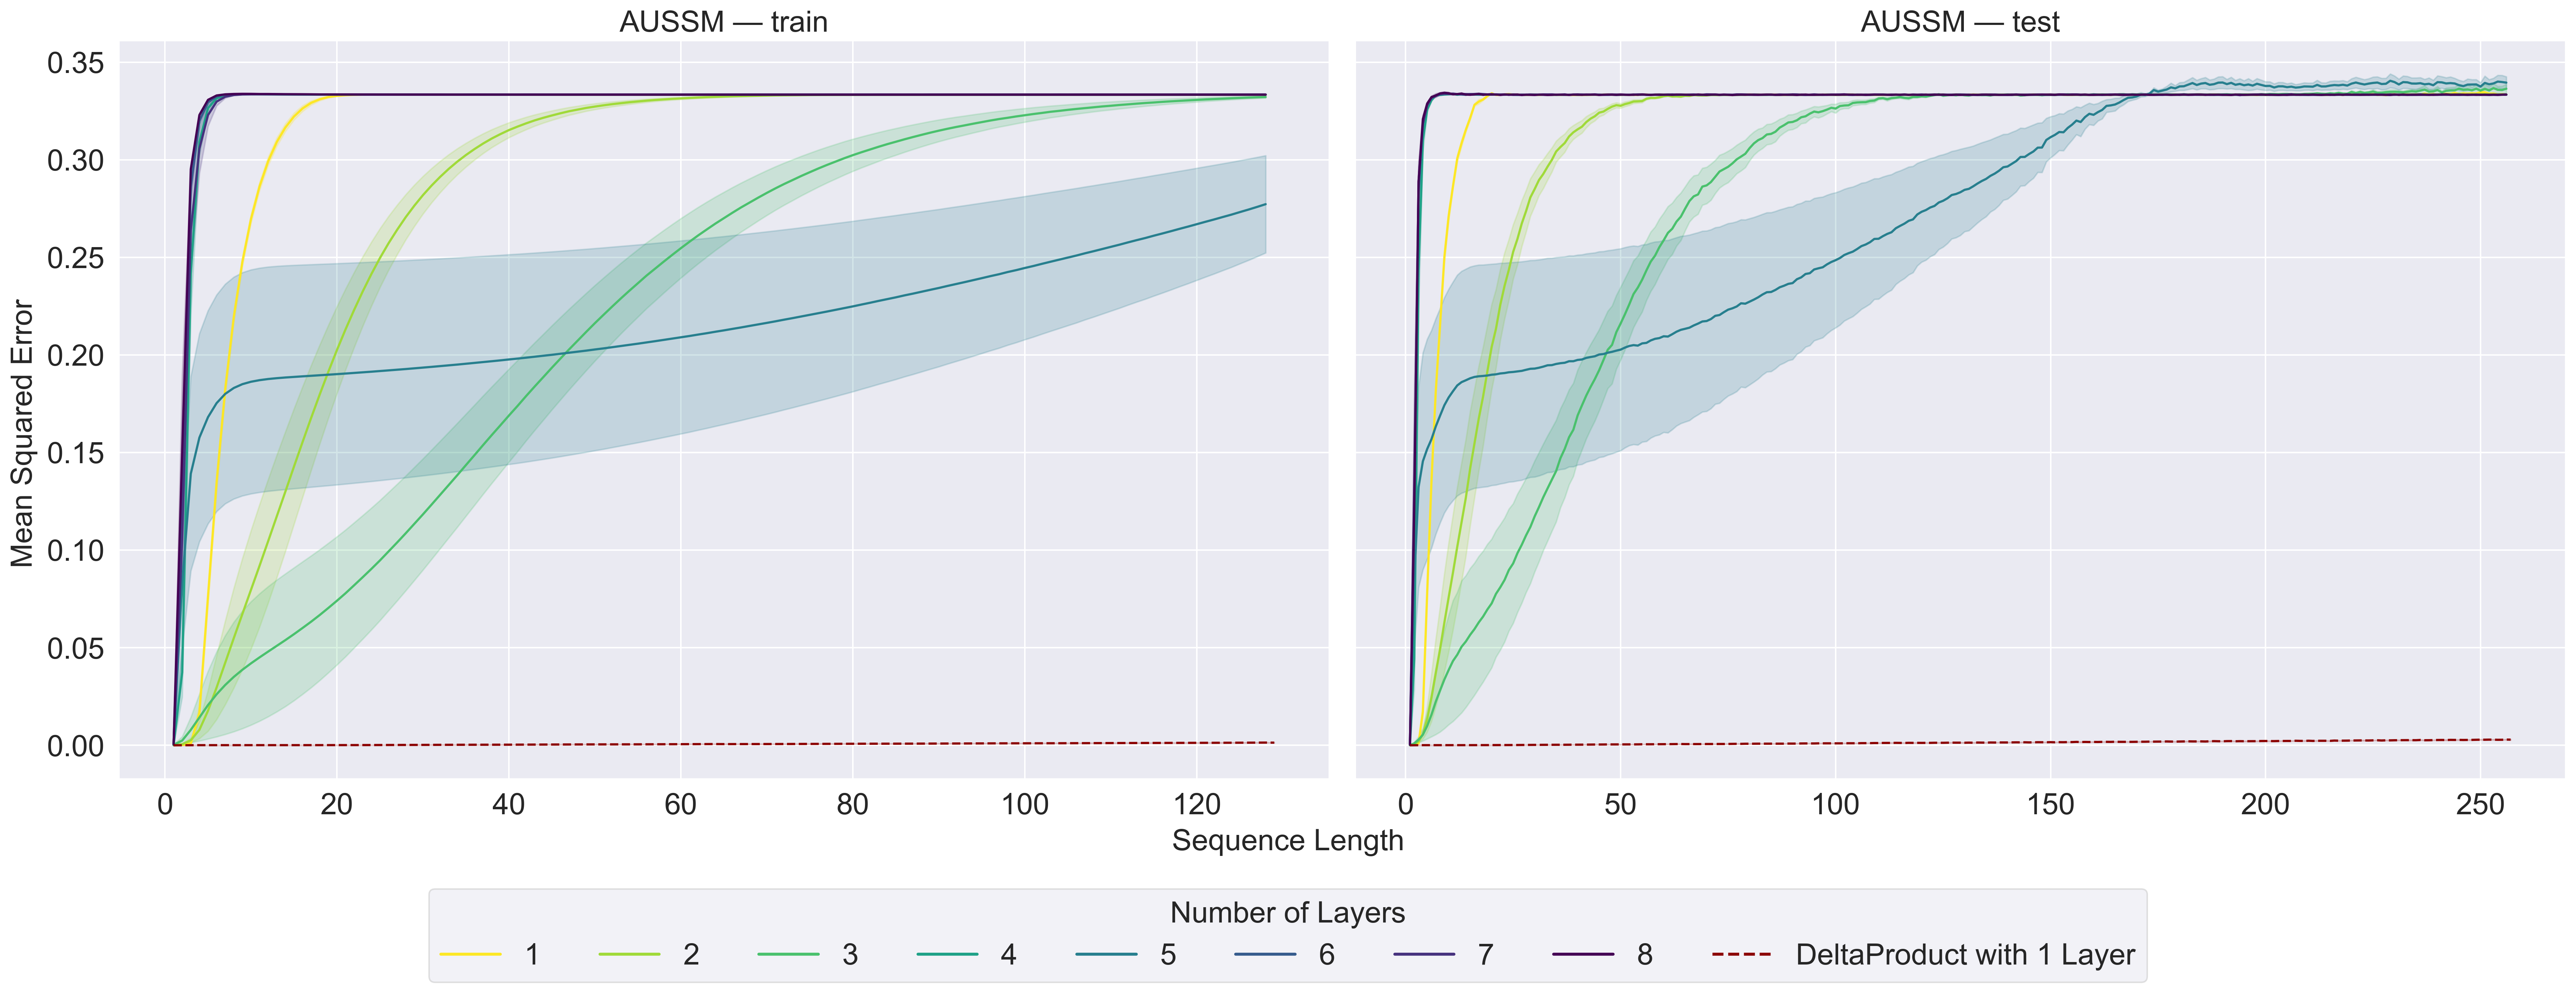
\includegraphics[width=0.95\columnwidth]{figures/mse_grid_aussm.png}
        \caption{Mean squared loss on the rotated vector prediction task at various sequence length for AUSSM, with different numbers of layers, on train (left) and test (right) sets. Standard error is shown using 3 seeds. Performance of DeltaProduct with 4 Householder products is shown as a reference.
}
        \label{fig:rotation_mse_aussm}
    \end{center}
\end{figure*}


\end{document}
